 \documentclass[11pt,a4paper]{report}
\usepackage[latin1]{inputenc}
\usepackage{csquotes}
\usepackage{amsmath}
\usepackage{mathtools}
\usepackage{pifont}
\usepackage{graphicx}
\usepackage{amsfonts}
\usepackage{amssymb}
\usepackage{fancyhdr}
\usepackage[left=4.5cm,right=4.5cm,top=4cm,bottom=2cm]{geometry}
\usepackage{listings}
\usepackage{color}
\usepackage{microtype}
\usepackage{booktabs}
\usepackage{chngcntr}
\usepackage{titlesec}
\usepackage{tikz}
\usepackage{float}
\usepackage{multicol}
\usepackage{tikz-qtree}
\usepackage{pgftree}
\usepackage{caption}
\usepackage{subcaption}
\usepackage{algorithm}
\usepackage{algpseudocode}
\usepackage[export]{adjustbox}
\usepackage[final]{pdfpages}
\usepackage{float}
\usepackage{caption}
\usepackage[square,sort,comma,numbers]{natbib}
\usepackage[super,negative]{nth}
\usepackage{url}
                  
\usetikzlibrary{arrows, automata}

\setcounter{secnumdepth}{5}
\setcounter{tocdepth}{5}

\newcommand{\quotes}[1]{``#1''}
\newcommand{\at}{\makeatletter @\makeatother}
\newcommand{\HRule}{\rule{\linewidth}{0.5mm}} 
\pagestyle{fancy}%
  \renewcommand{\headrulewidth}{0.3pt}
  \renewcommand{\footrulewidth}{0pt}
  \renewcommand{\chaptermark}[1]{\markboth{#1}{}}
  \renewcommand{\sectionmark}[1]{\markright{#1}{}}
  \fancyhf{}
  \fancyhead[LE,RO]{\sffamily\bfseries\thepage}
  \fancyhead[LO]{\sffamily\bfseries\rightmark}
  \fancyhead[RE]{\sffamily\bfseries\leftmark}
  \fancyfoot{}
\renewcommand*\thesection{\arabic{section}}  

%\setcounter{secnumdepth}{5}
\counterwithin{paragraph}{subsubsection}
\counterwithin{subparagraph}{paragraph}


\begin{document}

\pagenumbering{Roman} 

\begin{titlepage}
\begin{center}
% Upper part of the page
%\LARGE Uppsala University \\[1.5cm]
%\textsc{\Large Thesis Specification}\\[0.5cm]
% Title
%\HRule \\[0.4cm]
{ \huge \bfseries \textbf{ Evaluating the performance of a new aligner for ultra-short ancient DNA }}\\[0.4cm]
\HRule \\[0.5cm]
% Author and supervisor
\begin{minipage}{0.9\textwidth}
\begin{flushleft} \large
{\textbf{Homa Amini}}\\
% Homa.Amini.0062\at student.uu.se\\
\end{flushleft}
\end{minipage}
%\begin{minipage}{0.4\textwidth}
%\begin{flushright} \large
%\emph{Supervisor:\\Janet Kelso}\\
%kelso\at eva.mpg.de
%\end{flushright}
%\end{minipage}
\vfill
% Bottom of the page
%{Create: \large Oct 2015}\\
%{Last update: \large \today}
\end{center}
\end{titlepage}

\newpage\null\thispagestyle{empty}\newpage
\newpage
\newpage

\section*{Abstract}

Recent technological developments, such as high-throughput sequencing,
have enabled the sequencing of the genomes of many living organisms.  
Recently, it has also become possible to extract and sequence DNA from extinct organisms.\\ 
In comparison with modern DNA, the computational analysis of ancient DNA is complicated
by the fact that the sequenced fragments tend to be short, degraded and contaminated with
extraneous environmental sequences, such as bacteria and modern human DNA.

Identification of endogenous sequences from this mix of DNA is generally achieved by
alignment to a reference genome sequence. 
However existing alignment software does not work well with these ultra-short, 
chemically damaged sequences.

In order to deal with these much older samples a new software program has been implemented
(R-Candy; U. Stenzel unpubl.)which aims to align these ultra-short reads and cope with the high 
levels of chemical damage present, using self-index data structures for pattern matching
based on a Burrows-Wheeler Transform based FM-Index.

%It supports genomes of any size and requires not more than the provided genome size of memory.

This thesis evaluates the accuracy and performance of the R Candy aligner using 
simulated ancient DNA sequences. 

R Candy is compared to BWA, which is currently the most-commonly used aligner for ancient DNA.

Tests on simulated data showed that R-Candy outperforms BWA (run using default 
and ancient parameters), correctly aligning more endogenous reads correctly even
in the presence of extensive deamination, as well as incorrectly aligning fewer
microbial reads.

The current version of R-Candy compare to other aligners does not have a good 
throughput rate due to its backward search algorithm and non-supporting multithreading feature. 

\newpage\null\thispagestyle{empty}\newpage
\section*{Acknowledgements}
\newpage\null\thispagestyle{empty}\newpage

\tableofcontents
\newpage
\listoftables
\newpage
\listoffigures
\newpage

\pagenumbering{arabic} 



\section{Introduction} \label{Introduction}


There have been a number of breakthroughs in the development of sequencing 
technologies that allow us to now sequence whole genomes rapidly and at a 
reasonable cost\cite{NGS}\cite{454}\cite{NGS2}.
\\
These developments made it possible to get DNA from ancient organisms, 
including humans \cite{AncientDNA}\cite{fish2human}, and to sequence 
this DNA to learn about human history\cite{impactOFhg}\cite{ourGenome}
\cite{SNP}.

Since the primary goal of many studies is to find the genetic 
relationships between extinct and extant species, most often sequences 
from ancient organisms are analysed by aligning them to the genomes of 
closely related extant species\cite{Neanthertal}\cite{AncientDNA}.

A number of problems have to be addressed when ancient DNA is aligned.
The continuous maintenance of a living organism by enzymatic repair stops 
shortly after a death of a living organism. Along with the aggression of
microbes, insects and fungi on the DNA molecule make the extraction of a 
high-quality endogenous DNA very difficult and result in very short(the 
mean aDNA fragments vary between 36 to 150 base pairs providing by Illumina 
platform\cite{rizzi2012ancient} \footnote{This range varies due to environment 
and the age of the sample})and degraded DNA sequences\cite{paabo2004genetic}.
 
In addition to \emph{post-mortem} damage which is the degradation process of
ancient DNA over time results in deamination of cytosine to uracil and C to T 
changes at the both ends of DNA fragments \cite{futureofaDNA}, the low amount 
of survived endogenous DNA over a long period of time (above 38,000 years) 
are highly contaminated \cite{paabo2004genetic}\cite{aDNA}
by microbes, mostly bacteria of colonized dead organisms.

For samples that are reasonably preserved approaches to the alignment
of reads that are longer than 35bp have been developed. 
These use standard alignment software (eg BWA) but modify the parameters 
to compensate more differences.
But for older or less well-preserved samples that have even shorter 
sequences $(<35 bp)$ \cite{meyer2014mitochondrial},
using standard aligners like BWA leads to spurious alignments for a 
number of reasons.

First given the mammalian genome size - random alignments of shorter 
sequences become increasingly likely as the length decreases. 
This means that an increasing number of incorrect alignments can be 
found (and this is true for both endogenous and microbial DNA).

Second, standard aligners don't include a model of chemical damage that 
is specific to ancient DNA, and, therefore, penalise reads with mismatches
that are due to chemical damage.

Third, most aligners require an exact match of some minimum length(seed), 
that is often longer than the read length possible with ancient DNA.

Therefore, due to the lack of proper tools such as an aligner that is 
specific to ancient data and its characteristics, most of the generated 
data get discarded. 
This information reduction on the datasets of sparse endogenous data give 
us the motivation for a new aligner to efficiently analyze this particular
type of data.
\\
This thesis evaluates the performance of R-Candy aligner and compares it 
with BWA which is a widely used aligner for short reads.





%%%%%%%%%%%%%%%%%%%%%%%%%%%%%%%%%%%%%%%%%%%%%%%%%%%%%%%%%%%%%%%%%%%%%%%%%%%%%%%%%%%%%%%%%%%%%%%%%%%%
%%%%%%%%%%%%%%%%%%%%%%%%%%%%%%%%%%%%%%%%%%%%%%%%%%%%%%%%%%%%%%%%%%%%%%%%%%%%%%%%%%%%%%%%%%%%%%%%%%%

\clearpage
\section{Background } \label{Background }


\emph{Sequencing} is the process of determining the precise order of bases 
(adenine, guanine, cytosine, and thymine) that compose a DNA molecule. 
It is typically very hard to sequence a long fragment of a DNA molecule, 
such as a whole chromosome. However, It is easy to subdivide longer sequences
into short pieces, create multiple copies of them (called \emph{amplification} ) 
and sequence all the copies. The sequence of every piece is called a read and 
the whole process is known as shotgun sequencing \cite{makinen2015genome}.



The human genome sequence is made up of  3 billion DNA base pairs.
Although the human genome has been completely sequenced,it is not yet fully 
understood. However, some of the known characteristics of the human genome 
are CpG or CG poor and repeat-rich,$50 %$ of  the human genome is consists 
of repetitive DNA sequences.
The CpG sites are regions of DNA where a cytosine nucleotide is followed by 
a guanine nucleotide which are four folders under-represented in the human genome. 




\subsection{Ancient DNA } \label{Ancient DNA }
The ancient DNA exploration broadly describes as the retrieval of DNA sequences 
from fossils remains, archaeological discovery, museum specimens and other 
exceptional sources, only become doable when the new technologies for amplification
and sequencing of DNA sequences, called PCR got invented \cite{paabo2004genetic}.

The extracted DNA from long-dead organisms has significantly different characteristics
 that differ it from modern DNA which are summarized in Table\ref{aDNAchar} .\\



\begin{table}[H]
  \begin{tabular}{ |  p{4cm} | p{2cm} | p{5cm} |}
    \hline
  \textbf{  Properties} & \textbf{Modern DNA } &\textbf{ ancient DNA} \\ \hline
       Length &  100 bps  & $\leq$  35 bps \\ \hline
       Post-Morten substitutions & No  & Deamination of C$\to$T
(more likely near the end of a read) \\ \hline
  Contaminated & negligible & Microbial+Modern human\\ \hline
    \end{tabular}
\caption{Comparison between modern DNA and ancient DNA}
\label{aDNAchar}
\end{table}


The challenges with ancient DNA was the requirement for new software to efficiently 
align millions of ultra-short, degraded and deaminated reads to a reference genome.


\subsection{Alignment} \label{Alignment}

That sequence alignment is a common problem in computational biology, 
and one that can be simplified as follows:

An alignment between two strings $S_{1}$ and $S_{2}$ assumes a common origin and 
tries to highlight their similarities by explaining one of them as a small number 
of mutations, insertions and deletions applied to the other.\\

For those characters the survived over the times, an alignment of two strings is 
a list of indices (i,j) where $S_{1}[i]$ matches $S_{2}[j]$.\\ 
In its simplest form an alignment of two strings is obtained by placing two strings
one above the other one in the way that every character in either string is above 
a unique character in opposite string and then looking for relation between them.\\\\

As an example, consider the alignment of two strings $S_{1}$:\emph{'CCGATGA'} 
and $S_{2}$:\emph{'TCGCTG'} shown below. 

\begin{center}
	%\begin{tabular}{c *{12}c|cc|c}
	\begin{tabular}{ c c c |c| c c |c|c| c c|c| c c}
%	\hline
   $S_{1}$   &  & & C & C & G & A & - & T & G & A && \\
	%\hline
$S_{2}$ 	&  & &{\textcolor{red}T}& C & G & {\textcolor{green}-}& {\textcolor{cyan}C } 
 &  T & G & {\textcolor{green}- }& \\
    	                                 
	\end{tabular}
\end{center} 
In this alignment,there is one mismatch of character T highlighted in red, 
two deletion of character A highlighted in green and one insertion of character
C highlighted in cyan and all the other characters match their counterparts in 
the opposite string. 
\\\\

There are some key issues for an ideal alignment that needs to be considered:

\begin{itemize} 
	\item  What sort of alignment.
	\item  What kind of scoring system.
	\item  What algorithm to find the optimal alignment score.
\end{itemize}


\subsubsection{The Scoring Model} \label{The Scoring Model}

Comparing two sequences, we need a score to measure their similarity.
In the case of biological, the assumption is that the two sequences differ
due to a mutation process that led to a substitution 
of one base by another base,as well as insertion and deletion (INDEL) which add or remove bases.
We are aiming at aligning the two sequences in a way that maximizes their similarity.\\ \\
First, let me set up the problem with some notation:\\
We call the two sequences, $S_{1}$ and $S_{2}$ of length N and M respectively. 
The $i^{th}$ symbol in $S_{1}$ is $S_{1i}$ and $j^{th}$ symbol in $S_{2}$ is $S_{2j}$. 
In the case of DNA, these symbols are $\left\{A, C, G, T\right\}$.\\
$S(S_{1i}, S_{2j})$ is the score of aligning $S_{1i}$ to $S_{2j}$ (match or mismatch)
and $\delta$ is a penalty for introducing a gap by insertion or deletion of a character. 
Then the score of an alignment will be the sum of the substitution scores minus the 
penalties in it(the scoring system for our alignment is described in section 3.2.1.5 in more details).\\\\
As an example, the following is the substitution matrix for DNA sequence alignments.


\begin{table}[H]
 \centering
  \begin{tabular}{  c| r  r r  r }
    
  \textbf{  $S(S_{1i}, S_{2j})$ } & \textbf{A} &\textbf{ C} &\textbf{ G} &\textbf{ T} \\ \hline
       \textbf{A} &  1  & -1 & -0.5 & -1 \\
       \textbf{C} & -1  & 1 & -1 & -0.5 \\ 
       \textbf{G} & -0.5 & -1 & 1 & -1 \\ 
       \textbf{T} & -1 & -0.5 & -1 & 1
    \end{tabular}
%\caption{comparation between modern DNA and ancient DNA}
\label{alignment-exp}
\end{table}

If $\delta$=1 then the total score of following alignment is:
 
\begin{center}
	\begin{tabular}{c *{12}cccc}
%	\hline
        & & C & C & G & A & - & T & A & G && \\
	%\hline
 	  & & T  & C & G &  -  & C   &  T & -  & G & \\
    	                                 
	\end{tabular}
\end{center} 

-0.5 + 1 + 1 - 1 - 1 + 1 - 1 + 1 = 0.5

\subsubsection{Alignment Algorithms} \label{Alignment Algorithms}

Having the scoring system, we need an algorithm for finding the optimal alignment 
between a pair of sequences. Why we need a complicated heuristic algorithm and can
not just calculate the all possible alignments and choose the best one?\\
Because it is not computationally practical to calculate  
$$ \binom{2n}{n} = \frac{(2n)!}{(n!)^2} \simeq \frac{2^{2n}}{\sqrt{2\pi n}} $$
possible alignment between two sequences of length N. The problem gets even more complicated when we allow for gaps. 
The algorithm that guarantees to find the optimal alignment between a pair of sequences base on the best alignment 
score is an instance of dynamic programming. 
Dynamic programming has an essential role in computational sequence analysis.\\ 
For different types of alignment, there are slightly different types of dynamic programming algorithm(alignment algorithms).\\\\

The four essential steps in all dynamic programming algorithms are:

\begin{itemize} 
	\item Define a recursive structure for the optimal score\cite{eddydynamic}.
	\item  Create a  matrix for remembering the optimal score of subproblems \cite{eddydynamic}.	
	\item Fill the matrix by solving the  subproblems in a bottom-up approach\cite{eddydynamic}.
	\item Reconstruct the optimal approach that led us to the optimal score by a traceback on the matrix\cite{eddydynamic}.
\end{itemize}

In the following part I will describe the two more basic alignment algorithms that easily can be expanded to the more complex versions.

\paragraph{ Global alignment ( Needleman-Wunsch algorithm) }

The Needleman-Wunsch algorithm, which is based on dynamic programming is a widely used/well-known global alignment technique in biological sequence analyses to obtain the best-matching alignment of two sequences, allowing  gaps.\\
It aims to construct an optimal alignment using previous solutions for
optimal alignments of smaller subsequences \cite{durbin}.\\
We are going to calculate the optimal alignment score as been described in\cite{durbin} by constructing a matrix F indexed
by i and j, one index for each sequence, where the value F(i, j) is the score
of the best alignment between the initial segment $S-{1i..i}$ of $S_{1}$ up to $S_{1i}$ and the initial segment $S_{21..j}$ of $S_{2}$  up to $S_{2j}$. We can build F(i, j) recursively start by initialising F(0, 0) = 0. Afterwards we fill the matrix matrix from top left to bottom right. 
Once $ F(i-1, j-1 ), F(i-1 , j) $ and $ F(i , j-1) $ are known, we are able to calculate $ F(i, j)$ \cite{durbin}.

The best score of F(i,j) up to $S_{1i}$ and $S_{2j}$ is the maximum value of $S(i,j)$:

\[ F(i,j)= max
\begin{cases}
   F(i-1,j-1) + S(S_{1i} , S_{2j})\\
   F(i-1 , j)- \delta\\
   F(i,j-1)- \delta
\end{cases}
\]
The value in the last cell of matrix F(n,m) is by definition the optimal alignment score. 
For obtaining the alignment itself we need the path that led us to the final score. We use the traceback procedure to recursively recover the optimal alignment\cite{durbin}\cite{eddydynamic}.
We start from the last cell F(n,m) and follow each of the three cases that we chose to get to this point. We continue doing this until reaching the cell F(0,0) and in this point the optimal alignment is completely reconstructed \cite{eddydynamic}.



\paragraph{ Local alignment ( Smith-Waterman algorithm ) }

Compute the maximum scoring alignment of $L(S_{1}, S_{2})$ over all subsequences $S_{1}$ and $S_{2}$ is:


\[ F(i,j)= max
\begin{cases}
   F(i-1,j-1) + s(S_{1i} , S_{2j})\\
   F(i-1 , j)+ \delta\\
   F(i,j-1)+ \delta\\
   0 \quad  
\end{cases}
\]

To find the actual local alignment:
\begin{itemize}
 \item start at a cell with the maximum value.
 \item traceback.
 \item stop when you reach a cell with value 0.
\end{itemize} 



%%%%%%%%%%%%%%%%%%%%%%%%%%%%%%%%%%%%%%%%%%%%%%%%%%%%%%%%%%%%%%%%%%%%%%%%%%%%%%%%%%%%%%
\paragraph{Semi-global alignment}

Semi-global or "glocal" (short for global-local) algorithm is a combination of global
and local alignments. 
It is a practical strategy in the case of ancient DNA.
Aligning two sequences, one short ( an ancient DNA sequence) and the 
other one long( a chromosome sequence). In this case, neither global 
nor local alignment is completely applicable. The best solution here is to globally 
align the short sequence while only a local alignment is appropriate for the long sequence.


Having two sequences  $S_{1}$ and $S_{2}$, want to optimally align them.
$$S_{1}:ACACACTACCG$$
$$S_{2}:AGCACACA$$\\
%$s(S_{1i},S_{2j})= +2 \quad if \quad S_{1i} = S_{2j}(match) \quad and \quad-1  if \quad S_{1i}\neq S_{2j}(mismatch)$\\
%$s(S_{1i},S_{2j})= +2 $\quad if \quad $S_{1i} = S_{2j}(match)$ \quad and \quad-1 \quad if \quad $ S_{1i}\neq S_{2j}(mismatch)$\\

\[ F(i,j)= max
\begin{cases}
   s(S_{1i},S_{2j})= +2 \quad match \\
   s(S_{1i},S_{2j})= -1 \quad mismatch \\
  \delta = -1  \quad gap \enskip  penalty \\ 
\end{cases}
\] \\



$
H =\left
[
\begin{array}{ *{13}c} 
   & $\_$ & A & C & A & C & A & C & T & A & C & C & G \\
 $\_$  & \textcolor{cyan}{0} & 0 & 0 & 0 & 0 & 0 & 0 & 0 & 0 & 0 & 0 & 0 \\
 A & 0 & \textcolor{cyan}{2} & 1 & 2 & 1 & 2 & 1 & 1 & 2 & 1 & 0 & 0 \\
 G & 0 & \textcolor{cyan}{1} & 1 & 1 & 1 & 1 & 1 & 0 & 1 & 1 & 0 & 2 \\
 C & 0 & 1 & \textcolor{cyan}{3} & 2 & 3 & 2 & 3 & 2 & 1 & 3 & 3 & 2 \\
 A & 0 & 2 & 2 & \textcolor{cyan}{5} & 4 & 5 & 4 & 3 & 4 & 3 & 2 & 2 \\
 C & 0 & 1 & 4 & 4 & \textcolor{cyan}{7}  & 6 & 7 & 6 & 5 & 4 & 5 & 4 \\
 A & 0 & 2 & 3 & 6 & 6 & \textcolor{cyan}{9} & 8 & 7 & 8 & 7 & 6 & 5 \\
 C & 0 & 1 & 4 & 5 & 8 & 8 & \textcolor{cyan}{11} & \textcolor{cyan}{10} & 9 & 10 & 9 & 8 \\
 A & 0 & 2 & 3 & 6 & 7 & 10 & 10 & 10 & \textcolor{red}{12} & 11 & 10 & 9 \\
 \end{array} 
 \right]
$\\\\\\
Filling the matrix, the optimal alignment score will be the largest value
in the entire array.\\\\


$
T =\left
[ 
 \begin{array}{ *{13}c} 
       & $\_$ & A & C & A & C & A & C & T & A & C & C & G\\
  $\_$ & \textcolor{black}{0} & 0 & 0 & 0 & 0 & 0 & 0 & 0 & 0 & 0 & 0 & 0 \\
 A & 0 & \textcolor{red}{\nwarrow} & \leftarrow & \nwarrow & \leftarrow & \nwarrow & \leftarrow & \leftarrow & \nwarrow & \leftarrow & \leftarrow & \leftarrow \\
 G & 0 & \textcolor{red}{\uparrow} & \nwarrow & \uparrow & \nwarrow & \uparrow & \nwarrow & \nwarrow & \uparrow & \nwarrow & \leftarrow & \nwarrow \\
 C & 0 & \uparrow & \textcolor{red}{\nwarrow} & \leftarrow & \nwarrow & \leftarrow & \nwarrow & \leftarrow & \leftarrow & \nwarrow & \nwarrow & \leftarrow \\
 A & 0 & \nwarrow & \uparrow & \textcolor{red}{\nwarrow} & \leftarrow & \nwarrow & \leftarrow & \leftarrow & \nwarrow & \leftarrow & \leftarrow & \nwarrow \\
 C & 0 & \uparrow & \nwarrow & \uparrow & \textcolor{red}{\nwarrow} & \leftarrow & \nwarrow & \leftarrow & \leftarrow & \leftarrow &  \nwarrow & \nwarrow \\
 A & 0 & \nwarrow & \uparrow & \nwarrow & \uparrow & \textcolor{red}{\nwarrow} & \leftarrow & \leftarrow & \nwarrow & \leftarrow & \leftarrow & \leftarrow\\
 C & 0 & \uparrow & \nwarrow & \uparrow & \nwarrow & \leftarrow & \textcolor{red}{\nwarrow} & \textcolor{red}{\leftarrow} & \leftarrow & \nwarrow & \leftarrow & \leftarrow \\
 A & 0 & \nwarrow & \uparrow & \nwarrow & \uparrow & \nwarrow & \uparrow & \nwarrow & \textcolor{red}{\nwarrow}  & \leftarrow & \leftarrow & \leftarrow \\
 \end{array} 
\right]
$\\\\\\
The red path corresponds to the local alignment of the two sequences $S_{1}$ and $S_{2}$: 

$$S_{1}:A-CACAC\enskip TACCG$$
$$S_{2}:A\enskip G CACAC-A\enskip\enskip\enskip\enskip\enskip $$




Semi-global \footnote{Reads are globally aligned(fully aligned)where the reference is
locally aligned (with some gaps at the end of the reference string)} alignment results
have been produced by R-Candy as a result of mapping sets of short strings against 
long reference (for instance, strings of length $\geq 25$ bps aligned to a refernce of length 3.2 Gbs).
To calculate the highest similarity score(lowest Levenshtein distance) between two strings, 
we fill out the desirable and reference in the Y-axis and X-axis respectively.
Starting from the top left with score zero the score matrix leads us to the 
maximum score in the bottom right position.

Comparing every individual string with a corresponding-length reference is not feasible in
terms of memory consumption(exponential to the number of insertion and deletion allowance) 
therefore alternative heuristic which takes the following characteristics into account is needed: 


\begin{itemize}

\item Dealing with ancient DNA, we have very short reads and we do not allow for 
more than one INDEL, which reduces the memory usage.\\

\item 
In our case, the reference is a tree, not a sequence as our genome sequence is 
converted to a Wavelet Tree data structure.
We simply say that we split the reference into branches for reference. So we have
a reference that gives for any tree the outgoing edges from the root which all have 
letters  as a label and then an attached tree.
We will be able to start from the beginning (tree's root) and look for the query in 
branches which uses the Depth First Search(DFS) algorithm. 
It also is cheaper in terms of memory because using a tree as a reference makes
it reusable.
All needs to be done is to backtrack one step and look at another branch, so most
of the matrix is reused.\\


\item
As we always start from the root note:
\begin{enumerate}
 \item When we are done with the query it does not matter if its corresponding 
 reference if not finished yet.
 
 \item Not to end up at the leaf while the query has not finished yet,
we run down all the queries that are as long as our query.

\end{enumerate}

 \item Following the Branch and Bound heuristic, we increase the lower bound of the 
 introduced score that we are willing to endure. In the case of not finding anything 
 below that limit, no alignment found gets report.
 
\end{itemize}
Given a non-empty sequence $q\in (q_{1}..q_{n})$, we want to align it to 
another non-empty sequence (reference)$r\in (r_{1}..r_{n})$:\\\\



\begin{figure}[H]
\centering
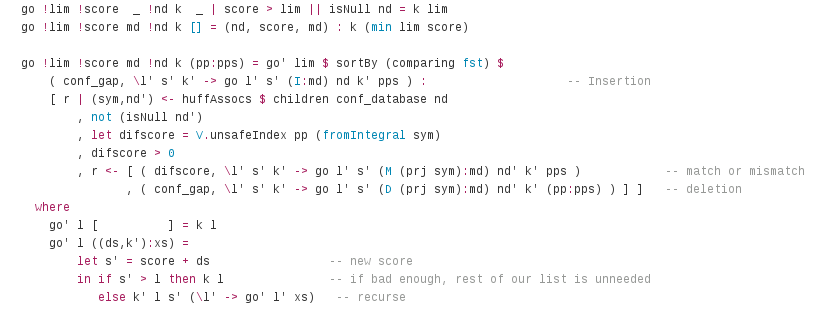
\includegraphics[width=15cm]{pictures/A_HS.png}
%\caption{ROC curve for simulated reads with deamination damage aligned to the simulated genome
 %        with deamination parameters.}
\label{formula}
\end{figure}


We take the minimal score of three options match/mismatch, insertion and 
deletions, as described in the above code.
The score that we have so far plus match score between q and r and pair it 
with Match operation (M) in the CIGAR field \cite{samtools}.\\
In the case of insertion (I) in the MD field \cite{samtools}: 
calculated score so far plus insertion score(penalty) pair with insertion
operation and CIGAR field for insertion.
The same procedure applied to deletion operation.

 
\paragraph{Scoring} \label{Scoring}

%\textbf{\emph{Going to rewrite this section, not my voice.}}
%But, this na\"{\i}ve definition of the correctness of an alignment has some 
%problems. For example after applying sequencing error and deamination damage on 
%the reads, the read does not exactly match the original genomic position. And 
%it would be a problem when the aligner chooses the location for a read with no or 
%fewer mismatches over the original location. In this case, the result will be 
%poorly judged as an incorrect mapping despite the more accurate matching position 
%has been chosen. The problem has been managed using mapping quality/alignment 
%score information. Such that a correct alignment of a read is defined as being 
%to its original genomic location and having the alignment score/mapping quality 
%lower/greater than a certain threshold. 
Let $\sigma$ and $\delta$ be the single stranded and the double stranded
deamination rates.  Let $l$ be the length of the read being aligned.  

For double stranded library preparation, let $\lambda$ be overhang
length parameter.  For every position $i \in [0..l-1]$ define

\begin{align*}
p_{fwd} &= \lambda^{i+1} \\
p_{rev} &= \lambda^{l-i} 
\end{align*}

For single stranded library preparation, let $\lambda_s$, $\kappa_s$ be
the 5' overhang length parameter and the 3' overhang parameter.  Let $l$
be the length of the read being aligned.  For every position $i \in
[0..l-1]$ define

\begin{align*}
p_{fwd} &= \lambda_s^{i+1} + \kappa_s^{l-i} - \lambda_s^{i+1} \kappa_s^{l-i} \\
p_{rev} &= 0
\end{align*}

Now define effective substitution probabilities

\begin{equation*}
p_{C} = \sigma p_{fwd} + \delta (1 - p_{fwd}), \quad
p_{G} = \sigma p_{rev} + \delta (1 - p_{rev}) 
\end{equation*}

Scoring a base at position $i$ with quality score $q$ involves
deamination, divergence and error.  We assume both a trivial error model
and a trivial model of evolution, where all possible changes occur with
a uniform rate derived from the quality score and a uniform rate given
by parameter $D$, respectively.  Define 

\begin{equation*}
\epsilon_0 = {10^{-q/10}}/4, \quad \epsilon = \epsilon_0 + D/3 - \epsilon_0 D/3
\end{equation*}

and the complete substitution matrix becomes (reference base in columns,
query base in rows, both in the order A, C, G, T):

\begin{equation*}
\left( \begin{array}{cccc}
1 - 3 \epsilon &       \epsilon                            &       \epsilon + p_{G} - 4 \epsilon p_{G} &       \epsilon \\
      \epsilon & 1 - 3 \epsilon - p_{C} + 4 \epsilon p_{C} &       \epsilon                            &       \epsilon \\
      \epsilon &       \epsilon                            & 1 - 3 \epsilon - p_{G} + 4 \epsilon p_{G} &       \epsilon \\
      \epsilon &       \epsilon + p_{C} - 4 \epsilon p_{C} &       \epsilon                            & 1 - 3 \epsilon 
\end{array} \right)
\end{equation*}

Alignment scores are simply the sum of the natural logarithms of the
entries in that matrix for every aligned base, plus a penalty for
insertions and deletions.  We use linear gap costs with a cost of $G$
per inserted or deleted base, where $G$ is a free parameter again.



%%%%%%%%%%%%%%%%%%%%%%%%%%%%%%%%%%%%%%%%%%%%%%%%%%%%%%%%%%%%%%%%%%%%%%%%%%%%%%%%%%%%%
\subsection{Data Structures}  \label{Data Structures}

Some of the main data structures used by our new aligner(R-Candy) for indexing and mapping process plus fundamental concepts required for better understanding of this thesis are described in this section. 

\subsubsection{Introductory} \label{Introductory}

\begin{table}[h]
 \centering
  \begin{tabular}{ | p{0.5cm} | p{0.5cm} | p{0.5cm} |p{0.5cm} |p{0.5cm} |p{0.5cm} |p{0.5cm} |p{0.5cm} |}
    \hline
  \textbf{b} & \textbf{a } &\textbf{r}  &\textbf{b} &\textbf{a} &\textbf{r} &\textbf{a} &\textbf{\$}\\ \hline
       0 & 1 &2&3&4&5&6&7 \\ \hline
      
   \end{tabular}
\caption{Array representation of "barbara" string}
\label{Array-representation}
\end{table}



A string \emph{S} is concatenation of \emph{N} characters. 
The length of the \emph{S} is denoted as $\lvert S \rvert$ = N and S[i] represents the $i_{th}$ character of the S.
The string's index starts from 0 and S[0,N-1] represents the whole string S while S[i..k] shows the substring of S from the position i to k inclusive with $i < k < N$. 
S[i..N-1] is the i\textsuperscript{th} suffix of So the 2th suffix of above example is S[2..7]='arbara\$' and
 S[0..i] is defined as i\textsuperscript{th} prefix, so the 7\textsuperscript{th} of table 2 is 'barbara\$'.
 
The pattern that we will be searching for is P.


$ \sum $  denotes the alphabet that all the characters of S belong to it And  $ c_{i} < c_{k}$ means $c_{i}$ appears before $c_{k}$ in lexicographic ordering.

A genome is presented by four letters $\left\{ 'A', 'C', 'G' and 'T'\right\}$, which corresponds to adenine, cytosine, guanine and thymine nucleotides. The character ('N') usually represents positions that are unknown in a genome.


A bit string is a string of characters called bits which are characters of a special alphabet  $ \sum = \left\{ 0, 1 \right\}$.
\\\\
%Since tree is another elementary data structure used in this thesis, I am going to explain it in more details.


A Trie is a rooted tree data structure with labeled edges by letters in the alphabet and nodes with concatenated characters from the root\cite{trie}. 

A Trie of all the suffixes of string S is called a Suffix Trie where each path from the root to a leaf is a suffix \cite{gusfield1997algorithms}.

Coalescing each non-branching path of a Suffix Trie into a single edge, labeled by the string of that path generates another kind of tree called Suffix Tree \cite{gusfield1997algorithms}.\\


Suffix Array was developed by Manber and Myers(1990) in order to reduce the memory requirement of suffix tree. In other words Suffix Array is a compact representation of Suffix Tree. \\
A suffix array for a string S[1..k], can be constructed like:
\begin{itemize} 
	\item  Construct all the suffixes of string S.
	\item  Alphabetically sort all these strings.
	\item Store all the starting indices of all these suffixes.
\end{itemize}
Figure 4 shows the construction of suffix array for string "barbara".
\begin{figure}[H]
\centering
\begin{subfigure}{.2\textwidth}
%  \centering
  %\includegraphics[width=.4\linewidth]
\textbf{SA}  \\
\enspace  \textbf{0}\quad barbara\$\\
\textbf{1}\quad arbara\$\\
\textbf{2}\quad rbara\$\\
\textbf{3}\quad  bara\$\\
\textbf{4}\quad   ara\$\\
\textbf{5}\quad     ra\$\\
\textbf{6}\quad     a\$\\
\textbf{7}\quad       \$
  \caption{All suffixes of string S}
  \label{fig:sub1}
\end{subfigure}%
\begin{subfigure}{.2\textwidth}
 % \centering
\textbf{$\xrightarrow{sort}$}
\label{fig:sub1}
\end{subfigure}%
\begin{subfigure}{.3\textwidth}
%  \centering
%  \includegraphics[width=.4\linewidth]{image1}
\textbf{SA} \\
\textbf{7}\quad \$\\
\textbf{6}\quad a\$\\
\textbf{4}\quad ara\$\\
\textbf{1}\quad arbara\$\\
\textbf{3}\quad bara\$\\
\textbf{0}\quad barbara\$\\
\textbf{5}\quad ra\$\\
\textbf{2}\quad rbara\$
 \caption{sorted  Lexicographically.}
  \label{fig:Burrows-Wheeler transform}
\end{subfigure}
\caption{Suffix array for string "barbara".}
\label{fig:test}
\end{figure}




%%%%%%%%%%%%%%%%%%%%%%%%%%%%%%%%%%%%%%%%%%%%%%%%%%%%%%%%%%%%%%%%%%%%%%%%%%%%%
\subsubsection{The Burrows-Wheeler Transform} \label{The Burrows-Wheeler Transform}

To index a reference genome in order to accelerate the process of finding the location of each read in the reference genome while aligning a read as well as using memory efficiently especially while working with a big data like human genome of ~3.2 Gbps (giga-basepairs), R-Candy uses Burrows-Wheeler Transform data structure.

The important role of BWT in pattern matching and indexing forced me to pay a special attention to BWT and its properties.Therefore, In this section, I describe the construction scheme of BWT and its special relation with Suffix Array.\\

\paragraph{Construction and Properties}

A Burrows-Wheelers transformation for a string S[0..L] is s special rearrangement of its characters into runs of similar called $S^{BWT}$ and consists of the following steps \cite{bwt}:

\begin{itemize} 
	\item Append special character \$ as a terminator symbol to the end of S which is lexicographically smaller than any other alphabet characters.
	\item  Construct all the cyclic rotations of S.
	\item  Lexicographically sort all these strings.
	\item The last column of this conceptual matrix \emph{$M_{T}$}, is called BWT(transformed text $S^{BWT}$).
\end{itemize}


For example, the BWT of string "barbara" is "arbbr\$aa", as shown in Figure \ref{barbaraBWT}.\\



\begin{figure}[H]
\centering
\begin{subfigure}{.5\textwidth}
  \centering
barbara\$\\
\$barbara\\
a\$barbar\\
ra\$barba\\
ara\$barb\\
bara\$bar\\
rbara\$ba\\
arbara\$b
%}
  \caption{All cyclic rotations for 'S'}
  \label{fig:barbaraBWT1}
\end{subfigure}%
\begin{subfigure}{.1\textwidth}
  \centering
$\xrightarrow{sort}$
\label{fig:sub1}
\end{subfigure}%
\begin{subfigure}{.5\textwidth}
  \centering
%  \includegraphics[width=.4\linewidth]{image1}
\$barbar\textcolor{red}{a}\\
a\$barba\textcolor{red}{r}\\
ara\$bar\textcolor{red}{b}\\
arbara\$\textcolor{red}{b}\\
bara\$ba\textcolor{red}{r}\\
barbara\textcolor{red}{\$}\\
ra\$barb\textcolor{red}{a}\\
rbara\$b\textcolor{red}{a}
 \caption{sorted  Lexicographically.}
  \label{fig:Burrows-Wheeler transform}
\end{subfigure}
\caption{Burrows-Wheeler transform for "barbara" string.}
\label{barbaraBWT}
\end{figure}








\begin{table}[h]
 \centering
  \begin{tabular}{ | p{0.5cm} | p{0.5cm} | p{0.5cm} |p{0.5cm} |p{0.5cm} |p{0.5cm} |p{0.5cm} |p{0.5cm} |}
    \hline
  \textbf{a} & \textbf{r} &\textbf{b}  &\textbf{b} &\textbf{r} &\textbf{\$} &\textbf{a} &\textbf{a}\\ \hline
       0 & 1 &2&3&4&5&6&7 \\ \hline
      
   \end{tabular}
\caption{Burrows-Wheelers transform of "barbara" string}
\label{BWT-barbara}
\end{table}


A key property of BWT is its special relationship with Suffix Array which is described below: \\
Adding a special terminating character \$ to the end of a string, all the $M^T$ rows will be suffixes of S. 
It makes a strong relation between suffix array built on S and the BWT matrix of S.\\
Let SA[i] denote the suffix at 0-based offset \emph{i} in SA(S) and BWT[i] denote the character 
at 0-based offset \emph{i} in BWT(S)\cite{bwt}, as can be seen in Table \ref{BWT&SA}.




\[ f(n)
\begin{cases}
    BWT[i]=S[SA[i]-1]   & \quad \text{if } SA[i] > 0\\
    \$  & \quad \text{if } SA[i]= 0\\
\end{cases}
\]


\begin{table}[h]
\centering
  \begin{tabular}{ c c l}
%  \begin{tabular}{| m{23pt} | m{23pt}| m{23pt}|}
  \textbf{  BWT} & \textbf{SA } & \\ 
       a 	&	 7	 &   \$\\  
       r 	&	 6	 &	 a\$ \\
       b 	&	 4	 &	 ara\$ \\
       b 	&	 1	 &	 arbara\$ \\
       r  	&	 3	 &	 bara\$ \\
      \$ 	&	 0	 &	 barbara\$ \\
       a 	&	 5	 &	 ra\$ \\
       a 	&	 2	 &	 rbara\$ \\

  \end{tabular}
  
\caption{The relation between BWT and SA}
\label{BWT&SA}
\end{table}


The other fascinating property of BWT that I describe here is called LF-mapping (last to first mapping).\\\\
\textbf{LF-mapping}  Last to first mapping describes the relation between the last(L) and first(F) column of $M_{T}$\cite{bwt}.\\\\
\textbf{Lemma 1:}\emph{the $i^{th}$ occurrence of c in the first column \emph{F} corresponds to the $i^{th}$ occurrence of the symbol c in the Last column \emph{L} of $M_{T}$} \cite{bwt}.\\\\
Figure \ref{Lemma1} illustrates Lemma 1\\

\begin{figure}[H]
\centering
\textcolor{cyan}{\$}barbar\textcolor{red}{$a_1$}\\
\textcolor{red}{$a_1$}\$barba\textcolor{green}{$r_1$}\\
\textcolor{red}{$a_2$}ra\$bar\textcolor{blue}{$b_1$}\\
\textcolor{red}{$a_3$}rbara\$\textcolor{blue}{$b_2$}\\
\textcolor{blue}{$b_1$}ara\$ba\textcolor{green}{$r_2$}\\
\textcolor{blue}{$b_2$}arbara\textcolor{cyan}{\$}\\
\textcolor{green}{$r_1$}a\$barb\textcolor{red}{$a_2$}\\
\textcolor{green}{$r_2$}bara\$b\textcolor{red}{$a_3$}
 \caption{Last to first property of BWT matrix}
 \label{Lemma1}
\end{figure}

To apply LF-mapping in efficient time of \emph{O(1}), a \emph{sum table} and an \emph{occurrence function }is needed.\\


\begin{itemize}

	\item C[c] is a table that for each character in the alphabet contains the total number of text characters that are alphabetically smaller than \emph{c} \cite{fmindex}.

	
	\item OCC(c,q) denotes:  The total number of occurrences of character c in the prefix L[1..q]\cite{fmindex}.It is possible to compute OCC(c, q) in constant time.
	%\item LF(.): Stands for Last-to-First column mapping.
	
\end{itemize}

Using \emph{OCC} and \emph{C}, the LF-mapping can be defined as \emph{LF(i) = C[L[i]] + OCC(L[i], i)} \\\\

\paragraph{Reversing}



We can use the First-Last property of BWT to reconstruct the original 
string. Start with \$ symbol on the first row and knowing if we go backward the 
character before \$ is $a_1$ and also using last to first property 
information. We know  $a_1$ has the same position as $a_1$ in the first 
column of the second row. Continue backward (if go backward in cyclic 
rotation) hit $r_1$. Apply the First-Last principle again and say this is 
the first occurrence of r, then we go to the  $r_1$ in the first column of 
$7^{th}$ row and continue using the First-Last property and then walk back 
one step and so on. We reconstructed the original string in reverse. By the 
knowledge of \$ ends the string, we walk clockwise in the cyclic rotation 
and have the original string.
 %LF(i)=C[T$^{bwt}$[i]]+Occ($T^{bwt}$[i],i).\\\\
BWT decompression Memory =  $\mathcal{O}(\lvert S \rvert)$ \\


%make tables if you had time%%%%%%%%%%%%%%%

\paragraph{Searching}
A search algorithm called backward search will be used for pattern recognition using $S^{BWT}$.\\

The BWT matrix is constructed by sorting all the cyclic rotations of a string,therefore
if a pattern \emph{P} appears in the string it will be a prefix in $M_{T}$ and if \emph {P} 
appears in multiple positions, they will be successive.\\ 
To search for a pattern using $S^{BWT}$, the backward search starts from the end of a pattern.
At first searches for an empty  pattern all over the BWT matrix. Then looks for the 
last character of the desired pattern. After finding the character, updates indexes and 
search for the character before that last one among the updated indexes.
Continues the process to find the pattern.Updating indexes is the crucial part of this procedure (See Figure \ref{backwardSearch}).\\\\




\begin{algorithm}[H]
   \caption{BWT matching algorithm}
    \begin{algorithmic}[1]
     % \Function{BWMatching}{$LastColumn,Pattern,FirstOccurance,Count$} 
      \Function{BWMatching}{$LastColumn,Patterns,C,OCC$}
       	\State ${top} = 0$
        \State ${bottom} = \lvert LastColumn \rvert -1$
        \While{ ${top}\le{bottom}$}
        	\If{$ Pattern  is  non  empty$}
            	\State $symbol = last letter in Pattern$
            	\State $remove last letter from Pattern$
        			\If {positions from top to bottom in LastColumn contain at least one occurrence of symbol}
        				\State $top = C(symbol)+ OCC(symbol,top-1)$
        				\State $bottom = C(symbol)+ OCC(Symbol,bottom)-1$
        			\Else
        				\State $output = 0 $
        			\EndIf
       		\Else 
       			\State $output = bottom-top+1 $ 
       \EndIf
     
     \EndWhile 
    \EndFunction

	\end{algorithmic}
\end{algorithm}




\begin{figure}[H]
\centering
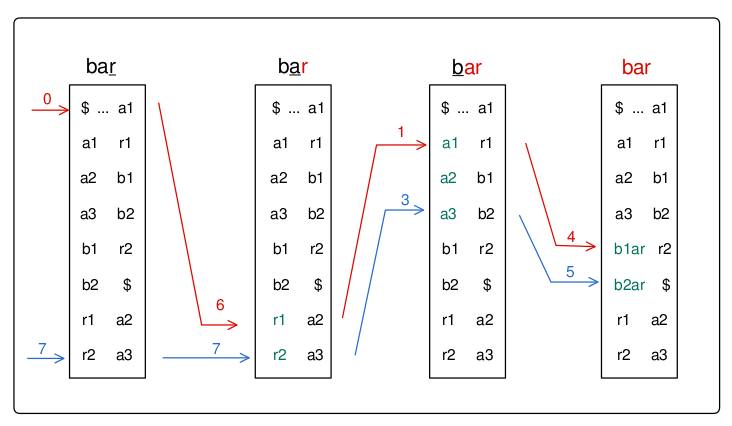
\includegraphics[width=12cm]{pictures/bar_1.png}
\caption{Backward search for pattern "bar" in string S using first and last column of BWT matrix. Updating indexes iteratively.}
\label{backwardSearch}
\end{figure}



\paragraph{Time Complexity}

The running time of the backward search on BWT depends on three factors; 
the length of the pattern P, the number of occurrence of P in the string and, 
more importantly, the access time of P in the suffix array.\\
The search algorithm consists of two phases, counting the number of occurrences of
a pattern and localization of their positions in the string.
The counting time is linear to the length of the P because at each iteration 
only one character of P is processed and length of the string doesn't have any 
impact on searching time which is one of the main reasons of using BWT for a large string like a genome.
On the other hand, the localization time is more affected by the number of occurrences 
of the pattern  because, for each occurrence of P, a look up at SA is needed.
\\\\

After introducing BWT and its properties and emphasising on its important job in pattern searching, in the following section the usage of BWT in an indexing data structure called FM-Index will be discussed\cite{fmindex}. 




%%%%%%%%%%%%%%%%%%%%%%%%%%%%%%%%%%%%%%%%%%%%%%%%%%%%%
\subsubsection{FM-Index (Full-text index)}  \label{FM-Index (Full-text index)}

Paolo Ferragina and Giovanni Manzini in 2000, six years after BWT was 
published invented a self-index data structure that combines BWT with some 
small auxiliary data structures. It allows to efficiently search for the 
occurrences of an arbitrary pattern P as a substring of the string S as well 
as locate the position of each occurrence. They named it FM-Index for Full-
Text Index in minute space where minute space emphasises on memory efficiency.
The FM-Index is consist of two parts. The first part keeps the number of
occurrence of a pattern in string S using the LF-mapping property of the BWT (Sum table \emph{C}). 
And the second part stores the location of patterns in S ( in our case we used a Suffix Array)\cite{Wavthesis}.\\

\textbf{Sum Table}  The sum table must be stored completely because the frequency of characters
are independent of each other and can cause memory consumption problem \cite{Wavthesis}.
But in  fact, the number of alphabets in a string are usually very small in comparison to
the length of the string, especially in the case of a genome which is an alphabet size of 
four or five in contrast to a length of millions.
\\

\textbf{Occurance Table} The crucial part of FM-Index that needs to be 
both time and memory efficient is occurrence data structure\cite{Wavthesis}.
There are different implementations of occurrence data structure all aim toward making it faster and more memory efficient.
\\

\textbf{Partial Suffix Array} A suffix array is needed to determine the exact position of each pattern in the string S.
But saving the whole SA is very memory consuming , therefore,
it is more efficient to just save part of SA and recover the rest
of it recursively to reach the saved positions at any time it is necessary \cite{Wavthesis}.\\


%%%%%%%%%%%%%%%%%%%%%%%%%%%%%%%%%%%%%%%%%%%%%%%%%%%%%%

\subsubsection{A Wavelet Tree based FM-Index} \label{A Wavelet Tree based FM-Index}

We used a Wavelet Tree based FM-Index to create a simple and robust index structure for 
a genome with efficient time complexity on pattern matching.\\

%\paragraph{Wavelet Tree}

A Wavelet Tree is a balanced binary tree to store strings as bit vectors in a 
compressed space\cite{navarroWavelet}\cite{Wavthesis}\cite{AlexBowe}.\\\\
Let s[0,n] be a binary sequence s[0,n] and $b \in {0,1}$ a finite alphabet. 
let $ rank_{b}(S, i)$ be the count of binaries b up to position i in string S 
and $ select_{c}(S,i)$  the position of $j_{th}$ occurrence of c in S.\\
The Wavelet tree is constructed recursively as follow:
\begin{enumerate}
    \item
		Take the string's alphabets and encode the first half of the alphabets as 0, and the second half as 1\cite {AlexBowe}:
    		$$\Sigma = \{ \$, a, b, r \}$$
			$$enc(\Sigma) = \{ 0, 0, 1, 1 \}$$
    \item
		Group each 0-encoded symbol, $\{ \$, a \}$, as a sub-tree;
    \item
		Group each 1-encoded symbol, $\{ b , r\}$, as a sub-tree;
    \item
		Repeat the procedure for each sub-tree until only one symbol has left.
\end{enumerate}
Wavelet tree for the string "Rhabarberbarbara" would look like this:
\begin{figure}[H]
\centering
\includegraphics[width=9cm]{pictures/wavelet.png}
%\includegraphics[width=0.75\textwidth, inner]{wavelet.png}
\caption{Wavelet tree for string "Rhabarberbarbara"}
\label{fig:barbWavlet}
\end{figure}

Construct the left subtree by taking all the 0-encoded symbols {\$,R,a,b} and
then divide them to new subtrees by re-encoding alphabet{0,0,1,1}.
Notice on the first level an "a" is encoded as a 0, but it is encoded as a 
1 on the second level and it becomes a 0 again at the leaf node.\\\\
The time complexity of Wavelet Tree to look for number of occurrences of a 
character up to specific position(OCC query) is $O(\log{}\mid\sum\mid)$.



%%%%%%%%%%%%%%%%%%%%%%%%%%%%%%%%%%%%%%%%%%%%%%%%%%%%%%%%%%%%%%%%%%%%%%%%%%%%%%%%


\subsubsection{Bi-directional Wavelet Tree}







%%%%%%%%%%%%%%%%%%%%%%%%%%%%%%%%%%%%%%%%%%%%%%%%%%%%%%%%%%%%%%%%%%%%%%%%%%%%%%%%
\subsection{Index Data Structure} \label{Index Data Structure}

There are some challenges on the mapping of short reads\\
The first challenge is time and memory consumption: aligning billions of short
reads to an enormous genome (human genome of size about 3,200 Mbps), 
calls for an efficient algorithm with optimal query time and memory space.\\
Therefore, R-Candy builds a robust index structure with 
the efficient time complexity for pattern matching in a long sequence of a genome
called a Wavelet Tree based FM-Index that lessens its time complexity and memory footprint for mapping . 
\\\\
An overview of R-Candy's data structure is presented in Figure \ref{DSOverview}\cite{Wavthesis}.\\

\begin{figure}[H]
\centering
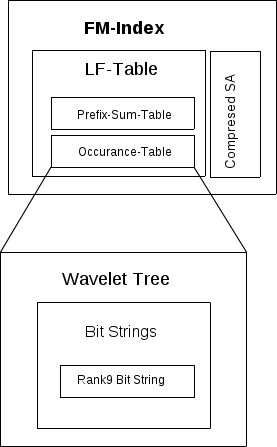
\includegraphics[width=4.75cm]{pictures/DSOverview2.png}
\caption{Overview of R-Candy's data structure }
\label{DSOverview}
\end{figure}


\subsubsection{Compressed Suffix Array} \label{Compressed Suffix Array}
The suffix array is needed to recover the position of patterns in the string
but storing the whole array is memory consuming, therefore, we used a
compressed version of SA to store some entries of SA.
The non-stored entries get retrieved by using LF-mapping.

\subsubsection{Prefix-Sum Table} \label{Prefix-Sum Table}
Prefix-Sum Table is a data structure used in FM-Index to store for every 
character c in string S the number of characters alphabetically smaller than c.

For the small alphabets of a genome, Prefix-Sum Table is stored
as a small array of alphabet size.

\subsubsection{Wavelet Tree}  \label{Wavelet Tree}
A Wavelet Tree data structure encodes a character string to a
binary tree recall Section 2.4.4.1.\\

Construction of a Wavelet-Tree for $ S_{BWT} $ of string 'barbara':

\begin{table}[h]
\centering
  \begin{tabular}{ c c c c c c c c}
%  \begin{tabular}{| m{23pt} | m{23pt}| m{23pt}|}
   a  & r & b & b & r & \$ & a & a \\ 
  \hline
   0 &	1 &	1 & 1 & 1 & 0 & 0 & 0\\  
  \hline
%  0 & 1  & 2 & 3 & 4 & 5 & 6 & 7   
  \end{tabular}
\caption{The Wavelet tree binary encoded root node for "barbara" BWT.}
\label{wavlet-binary-barbara}
\end{table}


\begin{figure}[H]
\centering
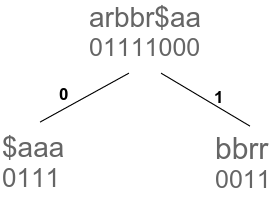
\includegraphics[width=4.75cm]{pictures/WavletBarbara.png}
\caption{Wavelet tree for "Rhabarberbarbara" string }
\label{Wavlet-barbara}
\end{figure}


A rank query can be done on  $O(\log{}\mid\sum\mid)$ time as is described below.
%After constructing the Wavelet tree (find at Figure 12), an rank query can be done on it. 

In order to calculate \emph{rank(5, a)} we use the following procedure
as illustrated in \ref{rank1}.\\
We know that \emph{enc(a)=1} at the root level by constructing wavelet
tree for the alphabet of  "Rhabarberbarbara" string.

\begin{enumerate}

    \item
		 Count the number of 1s in the range[1..7], at the root node, 
		 given by \emph{rank(7,0)=5 }. This is the index to query in 0-child.
		 
    \item
		As 'a' is encoded as 1 at this child, calculate \emph{rank(5,1)=4}. 
		We use 4 as an index for next branch.

    \item
		\emph{rank(4,0)=2} as 'a' is encoded as 0 here and return 2 as our
		 result since we are at the leaf node.

\end{enumerate}

\begin{figure}[H]
\centering
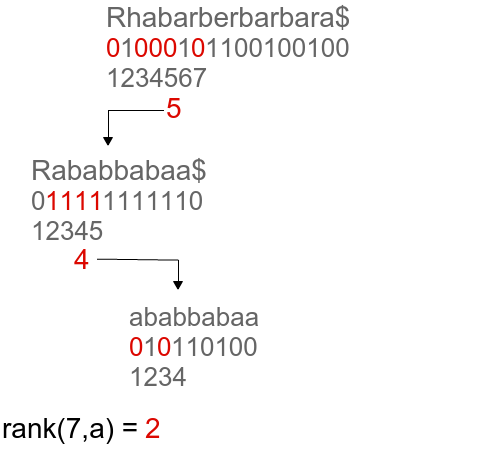
\includegraphics[width=7cm]{pictures/rank1.png}
\caption{The rank(7,a) over Wavelet tree for "Rhabarberbarbara" string }
\label{rank1}
\end{figure}

The space usage is given by this structure.
Bits proportional to the depth of  Wavelet tree are needed to encode
each character giving memory usage proportional to $H_{0}$(empirical entropy)\cite{entropy}.\\

We define \emph{$rank(n,0)= n- rank(n,1)$} and implement \emph{$rank(. , 1)$}
using the Rank9 structure described below.



%%%%%%%%%%%%%%%%%%%%%%%%%%%%%%%%%%%%%%%%%%%%%%%%%%%%%%%%%%%%%%%%%%%%%%%%%%%%%

\subsubsection{The rank9 Data Structure} \label{The rank9 Data Structure}

%In this part, the layout of our data structure will be introduced.\\	

The rank9 data structure was first proposed by Vigna, Sebastiano \cite{rank9}.
The main idea is to turn a bit sequence into a bit string that supports
rank queries in $O(1)$ time.\\

Consider an array of 64-bit words represented as bit array \emph{b}.
The bit at position p is stored in bit (\emph{p} mod 64) of
$ [p \backslash 64]$ \cite{rank9}.\\ 
Let a \emph{basic block} be a subsequence of eight words 
starting at bit position \emph{p}.\\
To construct the rank9  we divide the bit string into several basic
blocks and then divide these blocks further, into words of 64 bits.\\
We store the 512 bits in a \emph{basic block} and two words (as described in \cite{rank9}):

\begin{enumerate}

	\item The first word (first-level count) contains the total number of
	 1s till that position \emph{(rank(p)});
	
	\item The second one contains the seven 9-bit values (second-level counts)
	 \emph{rank(p + 64k)- rank(p)} , for 1 $\leq$ k $\leq$ 7,each shifted left by \emph{9(k-1)} bits.
	
\end{enumerate}

To construct the rank9  we divide the bit string into several basic blocks.
For each basic block boundary, a sum of previous ranks (first-level rank) and the address of  
stored offset values(second-level rank) are stored which gives us an efficient rank query time. \\

For each block, we store:\\\\
\centerline{$ block[i].total= rank(i*512)$}\\\\
\centerline{$ block[i].subtotal[j]= rank(i*512 + (j+1)*64)-block[i].total$}\\\\
\centerline{$ b[i*8]=raw[i*512..i*512+(k+1)*64)] $}\\\\
\centerline{$ OCC_{1}(x)=block[i].total+block[i].subtotal[j-1]+popcount(b[i*8 + j],0,k)$}



\[ where
\begin{cases}
	i=[ x \backslash 512 ]\\
	j=[(x \% 512 )\backslash 64 ]\\
	k=[ x \% 64  ]\\
\end{cases}
\]

%%%%%%%%%%%%%%%%%%%%%%%%%%%%%%%%%%%%%%%%%%%%%%%%%%%%%%%%%%%%%%%%%%%%%%%%%%%%

\subsection{Seeding Heuristics}

Set a limit on the number of allowed mismatches in the first few tens of bases
on a read sequence, calling it the \emph{seed} sequence.
By default, BWA uses the first 32 bps of a read sequence as a seed, allowing 
maximum two mismatches in order to increase the overall speed of the alignment 
(for reads that are shorter than 32 bps, the seed is disabled)\cite{bwa}. 
In the case of ancient DNA with high rates of mismatches at the 5-termini' and 
3'-termini due to the post-mortem deamination of cytosine, as well as also short 
read fragments, could limit the performance of seed-based alignment approaches 
to determine the genuine alignment .
The current version of R-Candy does not support the seeding strategy.


%%%%%%%%%%%%%%%%%%%%%%%%%%%%%%%%%%%%%%%%%%%%%%%%%%%%%%%%%%%%%%%%%%%%%%%%%%%%%
%%%%%%%%%%%%%%%%%%%%%%%%%%%%%%%%%%%%%%%%%%%%%%%%%%%%%%%%%%%%%%%%%%%%%%%%%%%%%


\section{Method} \label{Method}

In the past few years, the development of new DNA sequencing technologies made 
it possible to get DNA from ancient organisms.
The analysis of such a data regularly by aligning it to the genome of closely 
related modern species is a big challenge in human evolution studies.
A number of alignment software are developed to map such a dataset where 
simulated data is essential to guide the new software development and 
evaluating their performance.

Therefore, simulating data that captures the most crucial characteristics 
of real data is the key point in the evaluation of the new software.\\

To satisfy this, I developed a genome and NGS read simulation program to evaluate 
the performance of R-Candy in different cases.


%%%%%%%%%%%%%%%%%%%%%%%%%%%%%%%%%%%%%%%%%%%%%%%%%%%%%%%%%%%%%%%%%%%%%%%%%%

\subsection{Genome Simulation} 
\label{ Genome Simulation }

Generally, every genome consists of some repeated stretch of sequences which make 
the alignment of short reads from these repetitive parts very difficult due to 
finding the true alignment between the same repeated sequences.

In order to make the software evaluation more informative, we decided to first 
test the aligner with a simulated genome that has no short repeated sequences 
and check its accuracy and performance where we know the true alignment of each 
read.

In this thesis I used a probabilistic model called \emph{Markov Chain} model 
\footnote{More specifically \nth{1} Order Markov Chain as my future state only 
depends on my current state} to simulate a genome by generating stretch of 
nucleotides (A, C, G, T bases) in a way that  keeps the base composition of the 
real reference genome but not generates repeats.
 
 
A Markov chain graphically can be drawn as a collection of states, 
each corresponds to a particular nucleotide (A, C, G, T) with arrows
between them like the following (Figure \ref{MC}). 
\\\\ 
Having a set of states,  $ S= \{ A, C,  G, T \}$  and probability
parameter  associated with arrows in the figure which determines the
probability of transferring from one state to the next state (Transition)
or staying on the same state (Emission).

\begin{figure}
 \begin{center}
  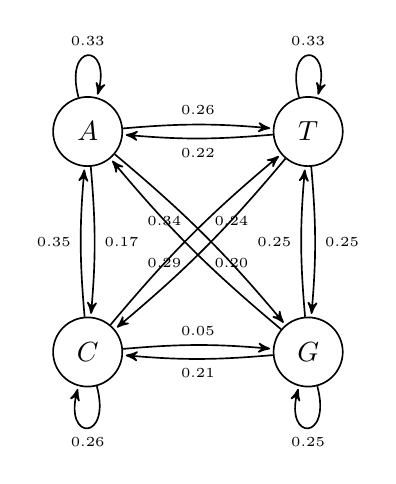
\begin{tikzpicture}[->,>=stealth',shorten >=1pt,auto,node distance=2.8cm,
                    semithick,bend angle=5]
   \tikzstyle{every state}=[fill=white,draw=black,text=black]

   \node[state]         (A)              {$A$};
   \node[state]         (T) [right of=A] {$T$};
   \node[state]         (C) [below of=A] {$C$};
   \node[state]         (G) [below of=T] {$G$};
  
   \path (A) edge [bend left]  node {\tiny 0.26} (T)
  			edge [loop above] node {\tiny 0.33} (A)
            edge [bend left]  node {\tiny 0.17} (C)
            edge [bend left]  node {\tiny 0.24} (G)
        (T) edge [loop above] node {\tiny 0.33} (T)
            edge [bend left]  node {\tiny 0.22} (A)
            edge [bend left]  node {\tiny 0.20} (C)
            edge [bend left]  node {\tiny 0.25} (G)
        (C) edge [bend left]  node {\tiny 0.34} (T)
            edge [loop below] node {\tiny 0.26} (C)
            edge [bend left]  node {\tiny 0.05} (G)
            edge [bend left]  node {\tiny 0.35} (A)
        (G) edge [loop below] node {\tiny 0.25} (G)
       	    edge [bend left]  node {\tiny 0.21} (C)
        	edge [bend left]  node {\tiny 0.29} (A)
            edge [bend left]  node {\tiny 0.25} (T);
  \end{tikzpicture}
  \caption{Trained \nth{1} order Markov chain based on human reference genome}
  \label{MC}
 \end{center}
\end{figure}





As mentioned above these probabilities are called \emph{transition or emission 
probabilities}, which are calculated by counting the number of state given its 
previous state ($ A \rightarrow A, A\rightarrow C, A \rightarrow T, A \rightarrow 
G, C \rightarrow C,$ ...) in the genome of interest; see the Table \ref{transition-table}
(Filled with human reference genome bases consistency).And then create a 
\emph{Transition Matrix} by calculating the frequency of seeing each transition,
as shown in Figure \ref{transition-matrix}.\\

\begin{table}[h]
  \begin{tabular}{ |  p{1cm} | p{2cm} | p{2cm} | p{2cm} | p{2cm} |}
    \hline
  	%\textbf{Type} & \textbf{Read length } &\textbf{Running time(s) } 
  	%&\textbf{Speed \hspace{35pt}(no. of reads/s)} \\ \hline
  	  
 	             & A   & C & G & T \\ \hline
      A  & 279630175  & 143865843 & 199830254 & 220834783 \\ \hline
 	  C	 & 207298683  & 148996334 & 28155478 & 199938031\\ \hline
 	  G	 & 169559114  & 121898050 & 149073778 & 144192413\\ \hline
 	  T  & 187672847  & 169629108  & 207663790 & 280419080\\ \hline
      
 	  
   \end{tabular}
%\caption{Transition number for a genome sequence of length 
%1G bp and chromosomes of length 250M bp.}
  \caption{Transition number for human reference genome}
 \label{transition-table}
\end{table}

%And then calculate the frequency of seeing each transition 
%called \emph{Transition Matrix}, as shown below.


\begin{figure}[H]
 \centering
\[
T = 
 \begin{pmatrix}
   &  A  & C & G & T  \\
 A & 0.331252 & 0.170425 & 0.236721 & 0.261603  \\
 C & 0.354727 & 0.254961 & 0.0481794 & 0.342132  \\
 G & 0.289982 & 0.208471 & 0.254948 & 0.246599  \\
 T & 0.221997 & 0.200653 & 0.245644 & 0.331706 \\
  
 \end{pmatrix}
\]
 \caption{Transition Matrix for human reference genome}
 \label{transition-matrix}
\end{figure}

Besides specifying the transition probabilities, the probability of starting 
state( state \emph{S} in the graph) is required. In our case as we don't have
special interest on starting from particular state all four state are equally 
probable to get started. And no specific probability for an end state defined as 
E because the sequence can end anywhere (Figure \ref{MC_SE}).


\begin{figure}
 \begin{center}
 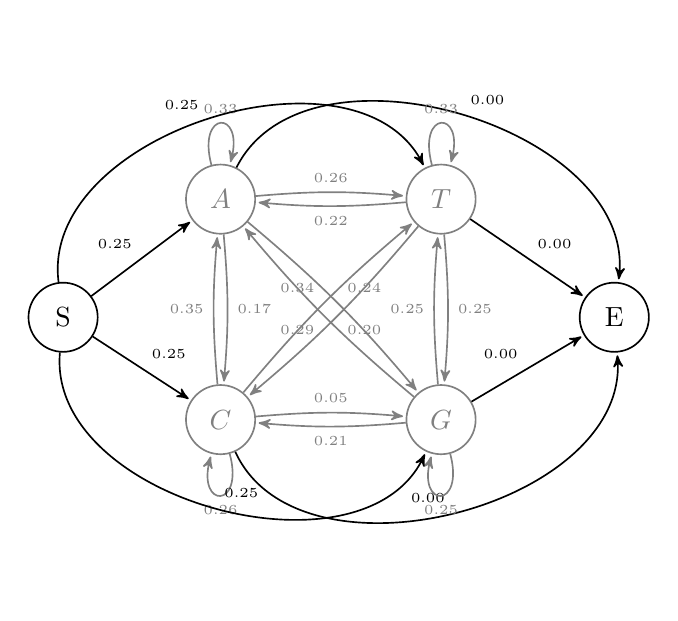
\begin{tikzpicture}[->,>=stealth',shorten >=1pt,auto,node distance=2.8cm,
                    semithick,bend angle=5]
  \tikzstyle{every state}=[fill=white,draw=gray,text=gray]

  \node[state]         (A)              {$A$};
  \node[state]         (T) [right of=A] {$T$};
  \node[state]         (C) [below of=A] {$C$};
  \node[state]         (G) [below of=T] {$G$};
  \node[state]         (S) [draw=black, text= black]at (-2,-1.5) {S};
  \node[state]         (E) [draw=black, text = black]at (5 ,-1.5) {E};
  
  \path (A) edge [gray, bend left]  node {\tiny 0.26} (T)
  			edge [gray, loop above] node {\tiny 0.33} (A)
            edge [gray, bend left]  node {\tiny 0.17} (C)
            edge [gray, bend left]  node {\tiny 0.24} (G)
            edge [bend left=80]  node {\tiny 0.00} (E)
        (T) edge [gray, loop above] node {\tiny 0.33} (T)
            edge [gray, bend left]  node {\tiny 0.22} (A)
            edge [gray, bend left]  node {\tiny 0.20} (C)
            edge [gray, bend left]  node {\tiny 0.25} (G)
            edge   			  node {\tiny 0.00} (E)
        (C) edge [gray, bend left]  node {\tiny 0.34} (T)
            edge [gray, loop below] node {\tiny 0.26} (C)
            edge [gray, bend left]  node {\tiny 0.05} (G)
            edge [gray, bend left]  node {\tiny 0.35} (A)
            edge [bend right=80]  node {\tiny 0.00} (E)
        (G) edge [gray, loop below] node {\tiny 0.25} (G)
       	    edge [gray, bend left]  node {\tiny 0.21} (C)
        	edge [gray, bend left]  node {\tiny 0.29} (A)
            edge [gray, bend left]  node {\tiny 0.25} (T)
            edge   			  node {\tiny 0.00} (E)
        (S) edge   			  node {\tiny 0.25} (A)
       	    edge   			  node {\tiny 0.25} (C)
        	edge [bend right=80]  node {\tiny 0.25} (G)
            edge [bend left=80]  node {\tiny 0.25} (T)
       
            ;
;
 \end{tikzpicture}
 \caption{Trained \nth{1} Order Markov-Chain based on human reference genome with start and end state}
 \label{MC_SE}
 \end{center}
\end{figure}


The simulation program asks for the length of the genome and then the Markov chain 
model starts randomly from one of the states and continuously walk between states 
based on their probabilities on transition matrix till the number of visited stateds 
is reached the given genome length which could equally be at any state. \\\\



%%%%%%%%%%%%%%%%%%%%%%%%%%%%%%%%%%%%%%%%%%%%%%%%%%%%%%%%%%%%%%%%%%%%%

\subsection{Read Simulation} \label{Read Simulation}

The second part of my test data preparation is about simulating ancient DNA reads 
sequenced by Illumina machine.



%%%%%%%%%%%%%%%%%%%%%%%%%%%%%%%%%%%%%%%%%%%%%%%%%%%%%%%%%%%%%%%%%%%

\subsubsection{Divergence} \label{Divergence}

By definition \emph{\quotes{ divergence is the separation
of a population's gene pool from the gene pools of other populations 
due to mutation, genetic drift, and selection \cite{divergence1}.}}\\

Introducing divergence property which also is used in R-Candy's mapping strategy 
is on top of simulated reads before any other source of substitution in my workflow. 

To understand how much divergence impedes mapping, I simulated reads with (0..N) 
number of absolute mismatches \footnote {These fix number of differences depends 
on the length of the read are representing different divergence rate. As an example 
2 mismatches on the sequence length 25 and 40 are showing the divergance rate of 8\% 
and 5\% respectively} to the reference genome.
And ran R-Candy with a default value for different datasets of reads with a 
different number of divergence substitution rates to evaluate the accurate of its 
alignment while aligning reads to close or far genomes.
 
 
%%%%%%%%%%%%%%%%%%%%%%%%%%%%%%%%%%%%%%%%%%%%%%%%%%%%%%%%%%%%%%%%%%%%%%%%%%%%%%%%%%%%%%%%%%%%%% 

\subsubsection{Sequencing Error} \label{Sequencing Error}
 

A sequencing error is an incorrect identification of a nucleotide base resulting 
to an inaccurate machine read. Due to the error in the base calling, there is no 
precise DNA sequencing. \\
A quality score indicating the confidence level of correctly seeing a base is 
assigned to each base of a read sequence.\\
Different sequencing platform have different quality score leading to variable 
sequencing error. These errors become visible when aligning a read to a reference 
string as substitutions or mismatches.\\
The main sequencing error for Illumina platform is base substitution due to 
reading out one base at a time \cite{art}.The substitution error probability is 
calculated by the base quality score along with the called base.\\

The output data of sequencing machines significantly differs in quality for 
several reasons ( for illustration, see Ewing et al. 1998) therefore, an effective 
measure for the reliability of such a data is vital \cite{phred1}.\\

In order to assess the accuracy of sequencing data, base calling accuracy by Phred 
quality score (Q score) is the most widely used metric. It demonstrates the probability 
of seeing an error in each bases, calling by a sequencer.\\

Phred quality scores are defined as \cite{phred2}:

$$ Q = -10  log_{10}P   $$
$$  or $$
$$ P = 10 ^ { \frac{-Q}{ 10 } } $$

For instance, if Phred score of a base is Q$=$40, it means the probability of an 
incorrect base call is a 1 in 10000 which shows 99.99\% base calling accuracy 
\cite{IlluminaPhred}. \\  

In order to implement sequencing error for simulated reads, There are two
options in my simulator (readSim):

The \textbf{first} option uses a next-generation sequencing read simulator 
(ART) to produce base quality and simulate sequencing error.


The \textbf{second} option for simulating sequencing error which is used for
my evaluation in this thesis is based on an empirical sequencing error profile 
data (in-house sequenced data).

The implementation looks at the quality values assigned to each base at each
position in the read and generates a distribution table for it (figure \ref{hist}).

\begin{figure}[H]
\centering
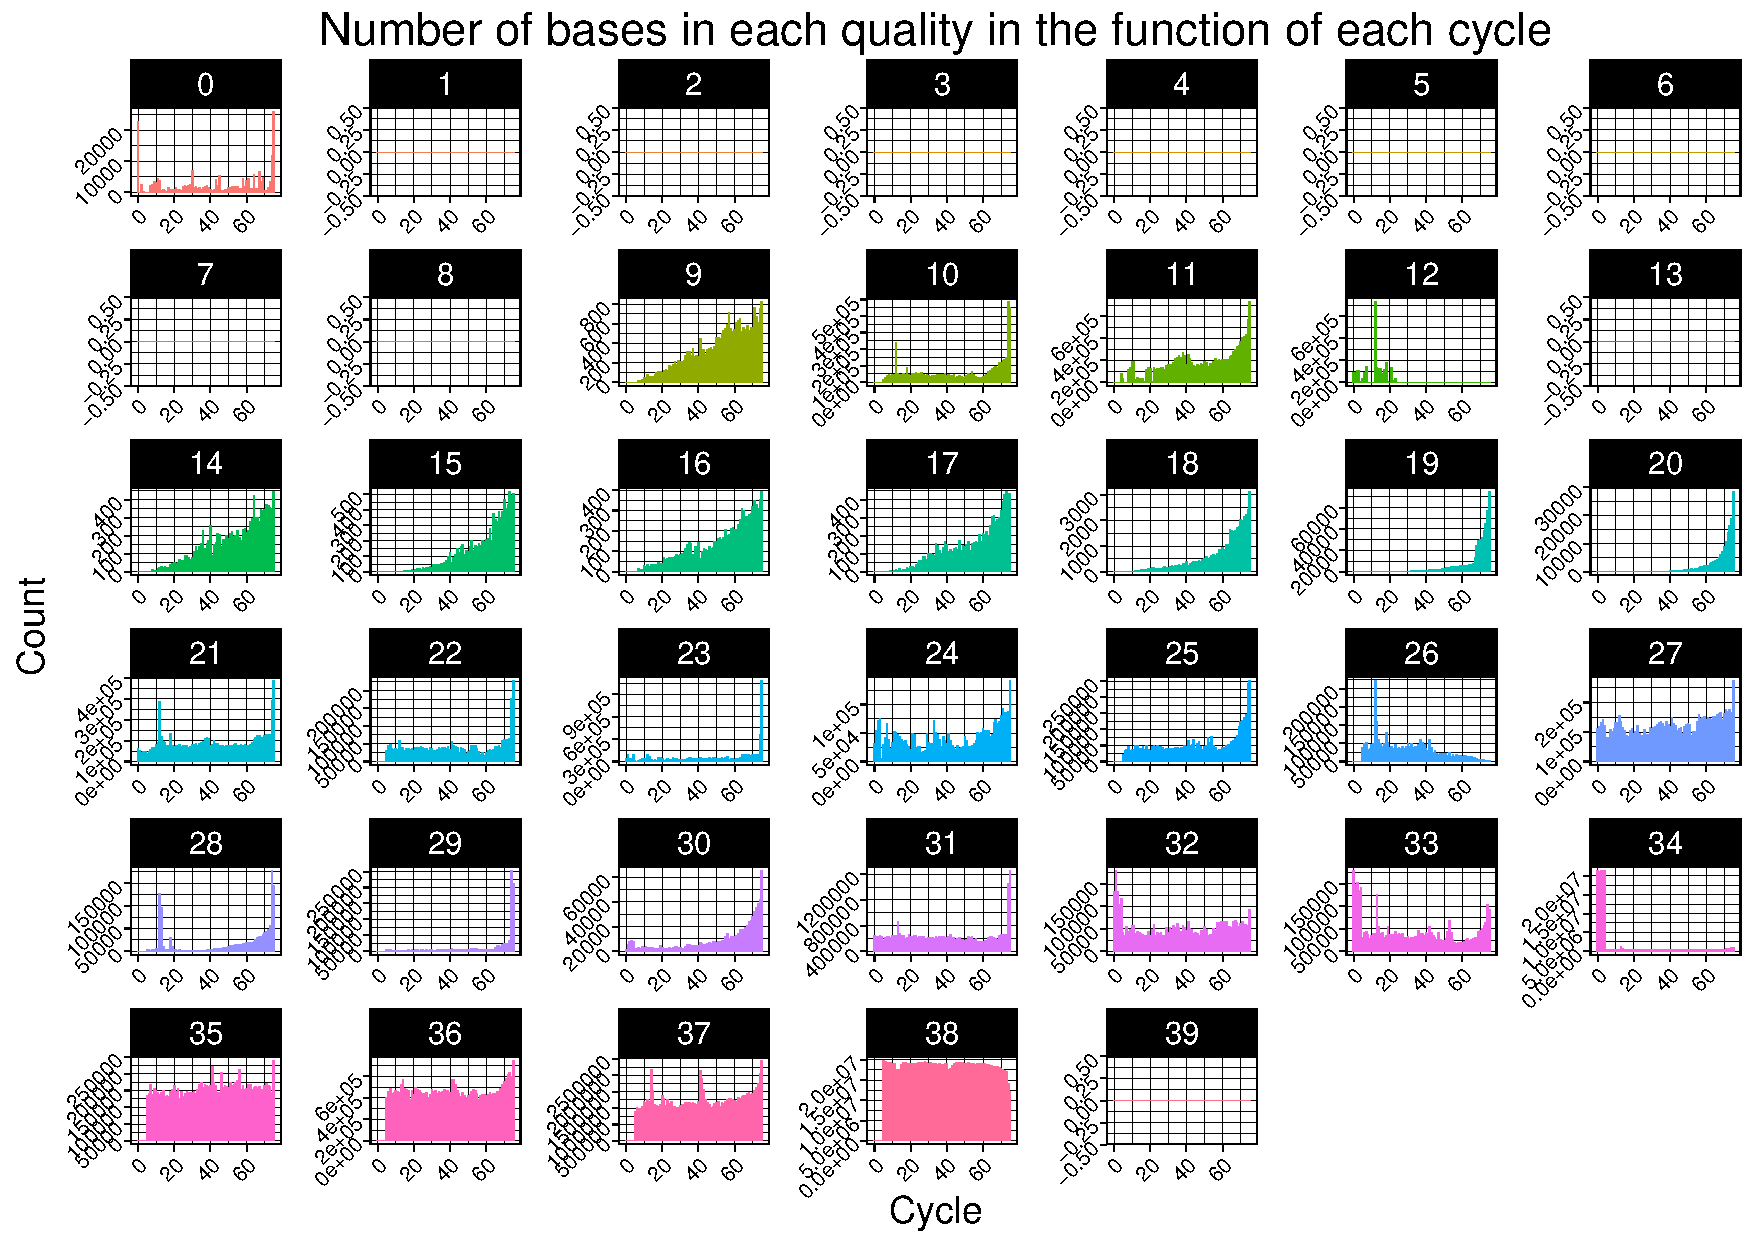
\includegraphics[width=12cm]{pictures/Rplot_quality.pdf}
\caption{Number of bases in each cycle in function of having certain quality}
\label{hist}
\end{figure}

Then calculates the probability mass function (PMF) which is the quality 
frequencies at each cycle for both forward and reverse reads. At the next 
step, cumulative distribution function (CDF) is calculated by summing up the 
quality frequency of each base with all quality bases before it (Figure \ref{CDF}).

\begin{figure}[H]
\centering
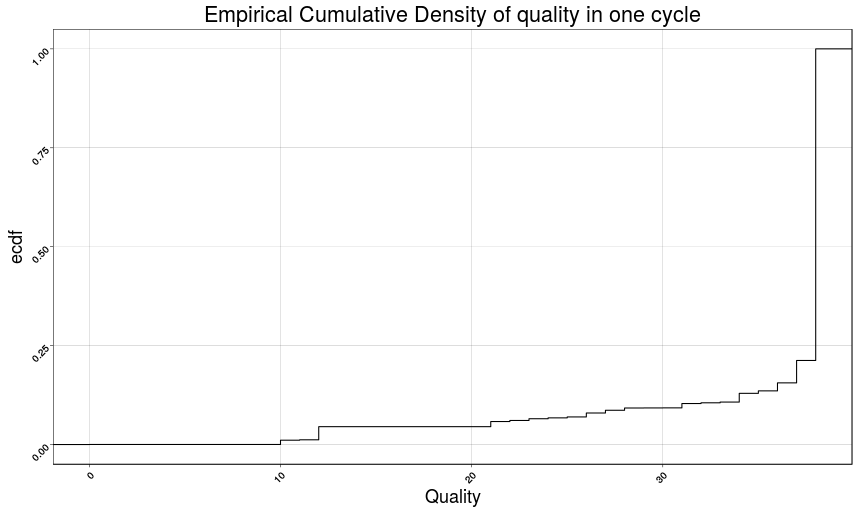
\includegraphics[width=12cm]{pictures/Rplot_ecdf.png}
\caption{Empirical cumulative distribution of all bases in cycle 11 of all forward 
reads}
\label{CDF}
\end{figure}

The quality score of each bases in a read, determined by a random number compare to 
its corresponding value in given CDF.

%%%%%%%%%%%%%%%%%%%%%%%%%%%%%%%%%%%%%%%%%%%%%%%%%%%%%%%%%%%%%%%%%%%%%%%%%%%%%%%%%

\subsubsection{Fresh DNA Reads Simulation} \label{Fresh DNA Reads Simulation}


Simulation of fresh DNA reads is done by extracting reads of given length from a 
reference genome and introducing a massive number differences to reads due to 
simulating different divergence (see also Section \ref{Divergence}) rate and on 
top of it sequencing errors of Illumina platform using empirical error profile 
is simulated (see Section \ref{Sequencing Error}).




%%%%%%%%%%%%%%%%%%%%%%%%%%%%%%%%%%%%%%%%%%%%%%%%%%%%%%%%%%%%%%%%%%%%%%%%%%%%%%%%%%

\subsubsection{Deamination} \label{Deamination}

A high nucleotide misincorporation rate of  deamination of cytosine(C) to uracil, 
code as thymine(T) are the unique characteristics of ancient DNA as the result 
of \emph{post-mortem} DNA damage\cite{mapdamage2}\cite{damagepattern}.\\ 

Observation in the recently introduced single-stranded library preparation protocol
has shown a significant increase in C to T substitution rates at the read terminals
\cite{mapdamage2}.\\

A computational model developed by Philip Jonson \cite{mapdamage2} is used to model
\emph{post-mortem} deamination behaviour as the followings:

For single stranded library preparation,
let $\sigma$ and $\sigma\prime $ be deamination rate in the 5' and 3' overhangs 
respectively and $\lambda$ be overhang length parameter. 

Let  $\delta$ and $l$ be the deamination rate at the middle(non-overhang) parts 
and the length of the read being aligned.\\

The DNA damage transition matrix is defined as:

$$ P_{dam} = 
 \begin{pmatrix}
  1 & 0 & 0 & 0 \\
  0 & 1-p_{ct} & 0 & p_{ct} \\
  0  & 0  & 1 & 0  \\
  0 & 0 & 0 & 1 
 \end{pmatrix}$$
 
Which columns and rows representing substitution rate between bases in reference 
and read respectivly.\\
The probability of damage for each base is defined as\cite{mapdamage2}:\\
%Where the base-specific damage probabilities are defined as\cite{mapdamage2}:\\
$$ p_{ct}(\sigma, \delta, \lambda, i) = ( \lambda_{i} \sigma + \delta(1 - \lambda_{i})) $$
 
It uses a geometric distribution to calculate the length of the overhang at both 
ends of a sequence based on certain deamination parameters.

The probability of being in overhang is provided by the user as the \emph{success 
fraction} value in the geometric cumulative distribution function (CDF).

Also for the simplicity we assume the probability of each base being in overhang 
and has the chance to be damaged is independent of the other bases. In other 
words, deaminating of one base has no influence on the other bases.\\

$$Pr( X=k ) = 1 - (1 - p)^{k}$$
$$ k = 1, 2, 3, ... $$


The simulation program first calculates the overhang length given the user-specified 
success fraction value.And then uses the user-specified substitution ratio numbers,
 $ \sigma $ and $\sigma\prime $, for substitution of the $ C \rightarrow T $ in 
overhangs which usually is higher than the deamination substitution ratio, $delta$, 
in non-overhang parts of aDNA reads.



%%%%%%%%%%%%%%%%%%%%%%%%%%%%%%%%%%%%%%%%%%%%%%%%%%%%%%%

\subsubsection{Ancient DNA Reads Simulation }  
\label{ Ancient DNA Reads Simulation}

Ancient DNA extracts consist of a low amount of endogenous DNA which used to be 
a big problem at evolution researchers until the recent technology of sequencing 
polymerase chain reaction (PCR) \cite{PCR} made it possible to amplify DNA 
sequences and produce high coverage data for deeper studies on human origins.
\\\\
readSim uses the following workfllow to simulate endogenous reads:
\begin{itemize}
 \item Uniformly sampled reads over the reference genome.

 \item Introducing a given number of differences to 
 reads in order to simulate different divergence rates.

 \item Simulating \emph{post-mortem} deamination damage based on deamination 
parameters (e.g overhang and non-overhang deamination rate in addition to 
probability of being in overhange) by users. 

 \item Adding the specific types of errors coming from sequencing machine based
on empirical cumulative distribution or ART .
\end{itemize}




%%%%%%%%%%%%%%%%%%%%%%%%%%%%%%%%%%%%%%%%%%%%%%%%%%%%%%%%%%

\subsubsection{Simulation of Microbial Reads } \label{Simulation of Microbial Reads }

Ancient DNA extracts are highly contaminated by mostly environmental microbes 
that always make the recognition of endogenous and exogenous DNA hard for aligners.
Although there is a database of known bacteria DNAs that could help us to detect 
bacterial sequences and don't mix them with endogenous DNA sequences but still 
there are a lot of unknown bacterial contamination.
\\\\
In order to have a realistic simulation of ancient DNA, we decided to simulate 
microbial DNA sequences besides our genomic DNA reads simulations.
\\\\
The microbial reads simulation process consist of:

\begin{itemize}

 \item Generating a totally random string of DNA nucleotides (A, C, G, T) for a 
given length (Chance of seeing each nucleotides is the same as the other one and 
eaqual to 0.25).

 \item Add the \emph{post-mortem} deamination damage to the reads which is the 
substitution of base Cytosine to base Thymine, given deamination parameters 
to simulate ancient damage on microbial sequences.


 \item Introducing sequencing errors to the simulated read.

\end{itemize}




%%%%%%%%%%%%%%%%%%%%%%%%%%%%%%%%%%%%%%%%%%%%%%%%%%%%%%%%%%%%%%%%%%%%%%%%%%%%%%%%%
\subsection{Evaluation Criteria} \label{Evaluation Criteria}

Evaluation of R-Candy is done based on three aspects, namely, 
the mapping accuracy, the throughput and memory footprint.

\begin{itemize}

 \item The mapping accuracy: mapping accuracy is divided into two parts, 
 sensitivity (true positive rate) and specificity (false positive rate).

 Reported sensitivity on simulated genome is the number of correctly mapped
 (mapped to the read's original position in the reference genome) 
endogenous genomic reads divided by the total of simulated endogenous reads 
knowing the true alignment of the reads and clear structure in the genome.
Sensitivity on the human genome which contains some repetitive elements,
all the multiple alignments are reported by R-Candy.
In the case of multiple hits, we chose one arbitrarily from the set of 
multiple best hits(reads with the best alignment score) otherwise 
an aligner could easily achieve a high TPR by reporting all the multiple 
hits with the best AS where the true alignment will definitely be among them.
Then check if the picked alignment hits the read's true genomic location.

Then the arbitrarily picked alignment is evaluated 
by aligned position given the known true position of the read.\\


Specificity is the number of aligned  microbial reads 
divided by the total number of  microbial reads.

 \item The aligner's throughput: the number of mapped reads per second(bps/sec).

 \item The memory footprint: the required memory by the tool for indexing 
the reference string, processing the reads and storing them. 

\end{itemize}
 


%%%%%%%%%%%%%%%%%%%%%%%%%%%%%%%%%%%%%%%%%%%%%%%%%%%%%%%%%%%%%%%%%%%%%%%%%%%%% 
%%%%%%%%%%%%%%%%%%%%%%%%%%%%%%%%%%%%%%%%%%%%%%%%%%%%%%%%%%%%%%%%%%%%%%%%%%%%%

\section{Results and Discussion} \label{Results and Discussion}

R-Candy is an alignment program for ultra short ancient DNA sequences 
(25-50 bps) based on BWT of the reference genome. It is  written in Haskell. 
It performs semi-global alignment for single reads, 
generates an alignment score and reports all possible hits for each read.
\\
We compared the performance of R-Candy to another aligner that 
uses the Burrows-Wheeler transform\cite{bwa} on a number of simulated 
datasets modeling different types of reads. 

BWA is a widely used aligner for short reads including ancient
DNA sequence reads.
It has been widely used as aligner for ancient DNA by increasing 
the number of mismatches and gaps allowed.  
However, it includes no model of ancient DNA damage, and is not 
particularly well-suited for alignment of very short reads.



%%%%%%%%%%%%%%%%%%%%%%%%%%%%%%%%%%%%%%%%%%%%%%%%%%%%%%%%%%%%%%%%

\subsubsection{Evaluation Scenarios} \label{Evaluation Scenarios}

A simulated genome is used for evaluation due to its structure and
clear expectations and results. 

Evaluation on a real genome is used to 
confirm the R-candy's behaviour on simulated genome despite the 
differences between the two genomes.

The accuracy of the aligners is evaluated as explained in Section
 \ref{Evaluation Criteria}.

To simulate a genome we used the human reference genome, version hg19,
as a training dataset and the \nth{1} Order Markov chain as a training 
model. The reads are sampled from the simulated genome and the human genome. 

\emph{Post-mortem} damage (deamination) is a specific characteristic of ancient 
DNA that none of existing aligners for short reads are taken into account except 
R-Candy.\\

Using the reference genome (simulated or the human genome) I simulated 
reads of lengths 25, 30, 35, and 40 with and without the deamination 
typical of ancient DNA, and aligned these back to its reference genome
(either a simulated genome or to the human genome) using BWA and R-Candy (as 
described in Table \ref{test-scenarios})

In addition to deamination, I also added a massive divergence rate in
the form of 0-6 mismatches and sequencing error (using empirical error profile).  

I also tested the accuracy of alignment in the presence of microbial reads of 
lengths 25, 30, 35 and 40 with and without the deamination typical of ancient DNA, 
and aligned these to the simulated genome or the human reference genome.



\begin{table}[H]
  \begin{tabular}{ | c| l |}
    \hline
 		                           &  \textbf{Description} \\\\ \hline
       \textbf{  Scenario 1 }  &  Simulated fresh DNA sequences extracted from a simulated \\
                               &  genome, aligned with default parameters. \\ \hline
       \textbf{  Scenario 2 }  &  Simulated fresh DNA sequences extracted from the human \\
                               &  genome and aligned with default parameters \\  \hline
       \textbf{  Scenario 3 }  &  Simulated ancient DNA sequences extracted from a simulated \\
                               &  genome and aligned without damage parameters. \\  \hline
       \textbf{  Scenario 4 }  &  Simulated ancient DNA sequences extracted from the human \\
                               &   genome and aligned with damage parameters. \\  \hline
       
    \end{tabular}
 %\caption{Evaluation scenarios}
\label{test-scenarios}
\end{table}



%%%%%%%%%%%%%%%%%%%%%%%%%%%%%%%%%%%%%%%%%%%%%%%%%%%%%%%%%%%%%%%%%%%%%%%%%

\subsection{Evaluation on Simulated Fresh DNA Reads } \label{Simulated Fresh DNA Reads }
 
 \subsubsection {Alignment of Simulated Fresh DNA Reads to a Simulated Genome.}
 \label {Alignment of Simulated Fresh DNA Reads to a Simulated Genome.}
 
  \begin{itemize}

   \item \textbf{Data:} Simulated fresh DNA extracted from a simulated genome 
   with between 0 and 6 substitutions to allow increasing sequence divergence
   and including sequencing error generated from empirical quality distribution data.
 
   
   \item \textbf{Reference genome:} Reads were aligned to a simulated genome of 
length 1Gb.

    \item \textbf{Aligners:} 
R-Candy with default parameters and alignments score cut-off of 20. \\
BWA version 0.5.10-evan.10 with default parameters and ancient parameters 
\cite{green2010draft} (the number of mismatches 
(0.01) and the number of gap opens (2)).

  \end{itemize}
 
Here we aim to evaluate the performance of R-Candy on fresh DNA reads 
without using the deamination parameters (R-Candy's default parameters).

\begin{figure}[H]
\centering
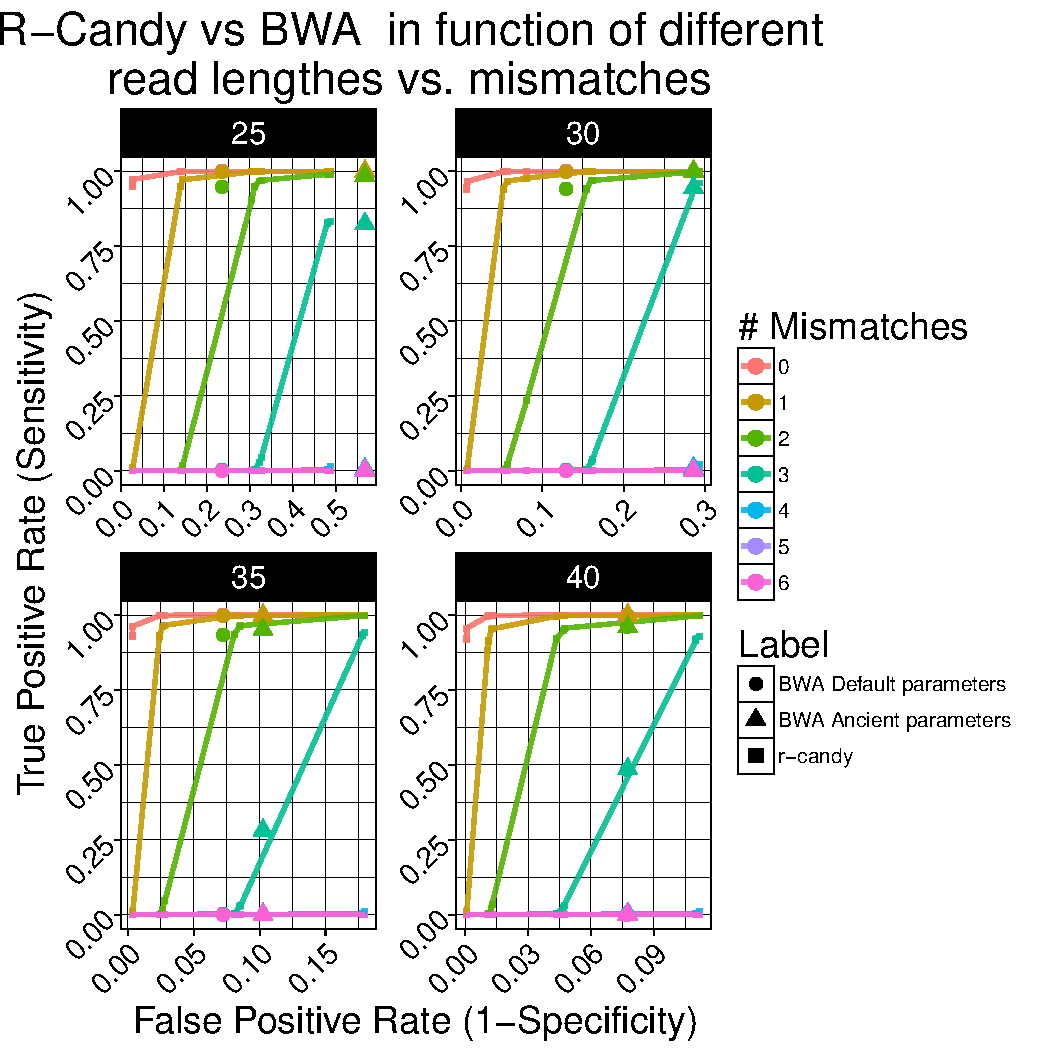
\includegraphics[width=12cm]{pictures/ROC_DS3_emp.pdf}

\caption{
ROC curve for the alignment to the simulated reference genome of simulated fresh 
sequence reads of lengths 25-40bp with between 0 and 6 substitutions due 
to increasing sequence divergence and empirical sequencing error.}

\label{DS3_emp}
\end{figure}


%%%%%%%%%%%%%%%%%%%%%%%%%%%%%%%%%%%%%%%%%%%%%%%%%%%%%%%%%%%%%%%%%%%%%%%%%%%%%%%%%%%%%%%

\subsubsection{ Alignment of Simulated Fresh DNA Reads to a the Human Reference Genome.}
\label{ Alignment of Simulated Fresh DNA Reads to a the Human Reference Genome.}

 \begin{itemize}
 
   \item \textbf{Data:} Simulated fresh DNA extracted from a simulated genome 
   with between 0 and 6 substitutions to allow increasing sequence divergence
   and including sequencing error generated from empirical quality distribution data.
   
   \item \textbf{Reference genome:} Reads were aligned to the human genome (version hg19) of length 3.2 Gb.

    \item \textbf{Aligners:} 
R-Candy with default parameters and alignments score cut-off of 20. \\
BWA version 0.5.10-evan.10 with default parameters and ancient parameters 
\cite{green2010draft} (the number of mismatches 
(0.01) and the number of gap opens (2)).


Here we aim to evaluate the performance of R-Candy on fresh DNA reads, 
aligned to the human reference genome without using the deamination parameters  
(R-Candy's default parameters).


\begin{figure}[H]
\centering
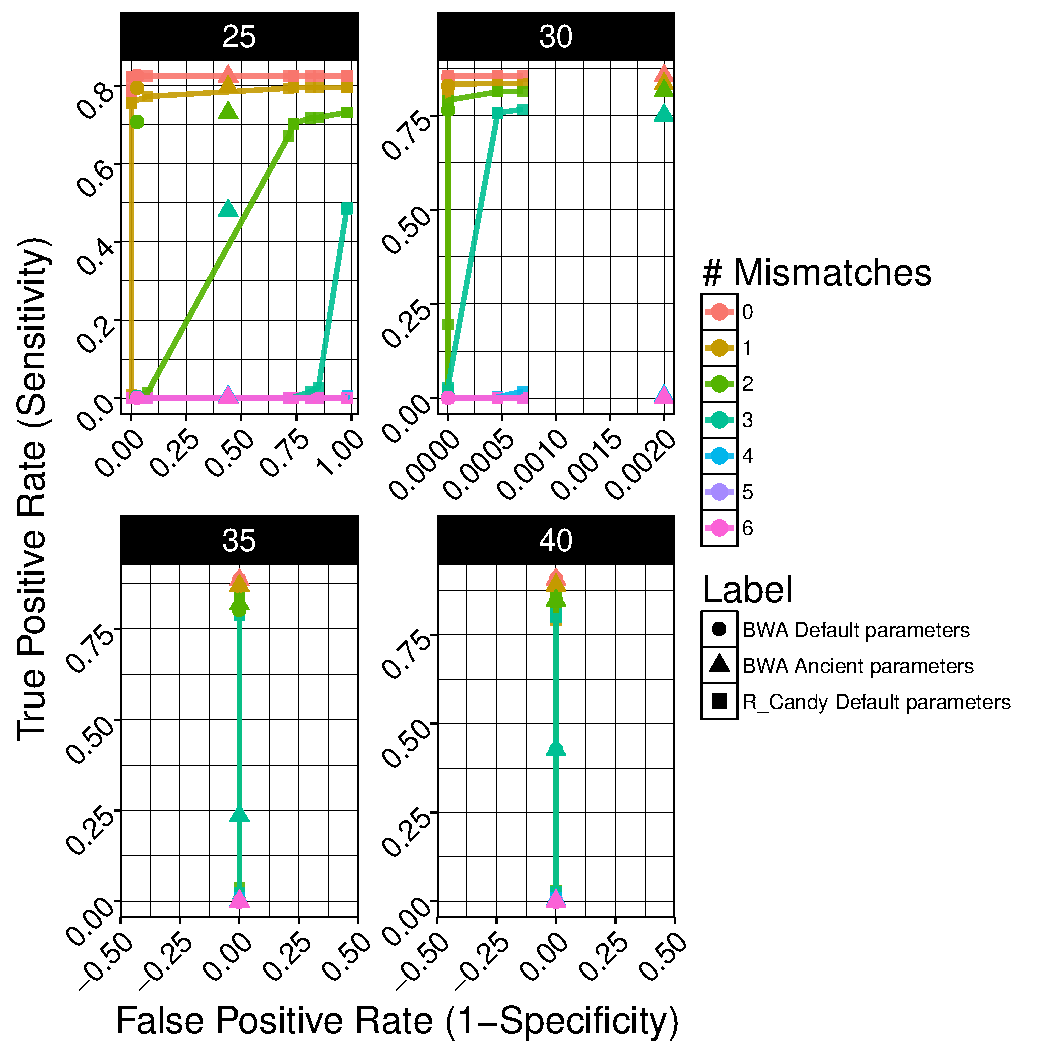
\includegraphics[width=12cm]{pictures/bROC_DS6_emp.pdf}

\caption{
ROC curve for the alignment to the human reference genome of simulated fresh 
sequence reads of lengths 25-40bp with between 0 and 6 substitutions due 
to increasing sequence divergence and empirical sequencing error.
}


\label{DS6_emp}
\end{figure}
  \end{itemize}



%%%%%%%%%%%%%%%%%%%%%%%%%%%%%%%%%%%%%%%%%%%%%%%%%%%%%%%%%%%%%%%%%%%%%%%%%%%%%%

\subsection{Evaluation on Simulated Ancient DNA Reads}

\subsubsection{Alignment of Simulated Ancient DNA Reads to a Simulated Genome.}
\label{ Alignment of Simulated Ancient DNA Reads to a Simulated Genome.}

\begin{itemize}
 
   
    \item \textbf{Data:} Simulated ancient DNA 
     with the following damage parameters $ \sigma = 0.9$, 
    $ \sigma\prime = 0.93 $, $\delta = 0.02 $,  and $\lambda = 0.3 $ and 
    between 0 and 6 substitutions to allow increasing sequence divergence
    including sequencing error generated from empirical quality distribution data
    extracted from a simulated genome.
  
 

  \item \textbf{Reference genome:}  Reads were aligned to a simulated genome of 
length 1 Gb.


  \item \textbf{Aligners:} R-Candy with ancient parameters 
  (-l left overhang parameter= 0.3, -r right overhang parameter= 0.3 , 
-d deamination rate in double stranded section = 0.02 , 
-s deamination rate in single stranded section = 0.9 )
  and cut-off alignments score 20. \\
  BWA with default parameters and ancient parameters \cite{green2010draft}
   ( number of mismatches ( -n 0.01 ) and the number of gap opening ( -o 2))

  \end{itemize}


Here we aim to evaluate the performance of R-Candy on ancient DNA reads
with deamination parameters.


\begin{figure}[H]
\centering
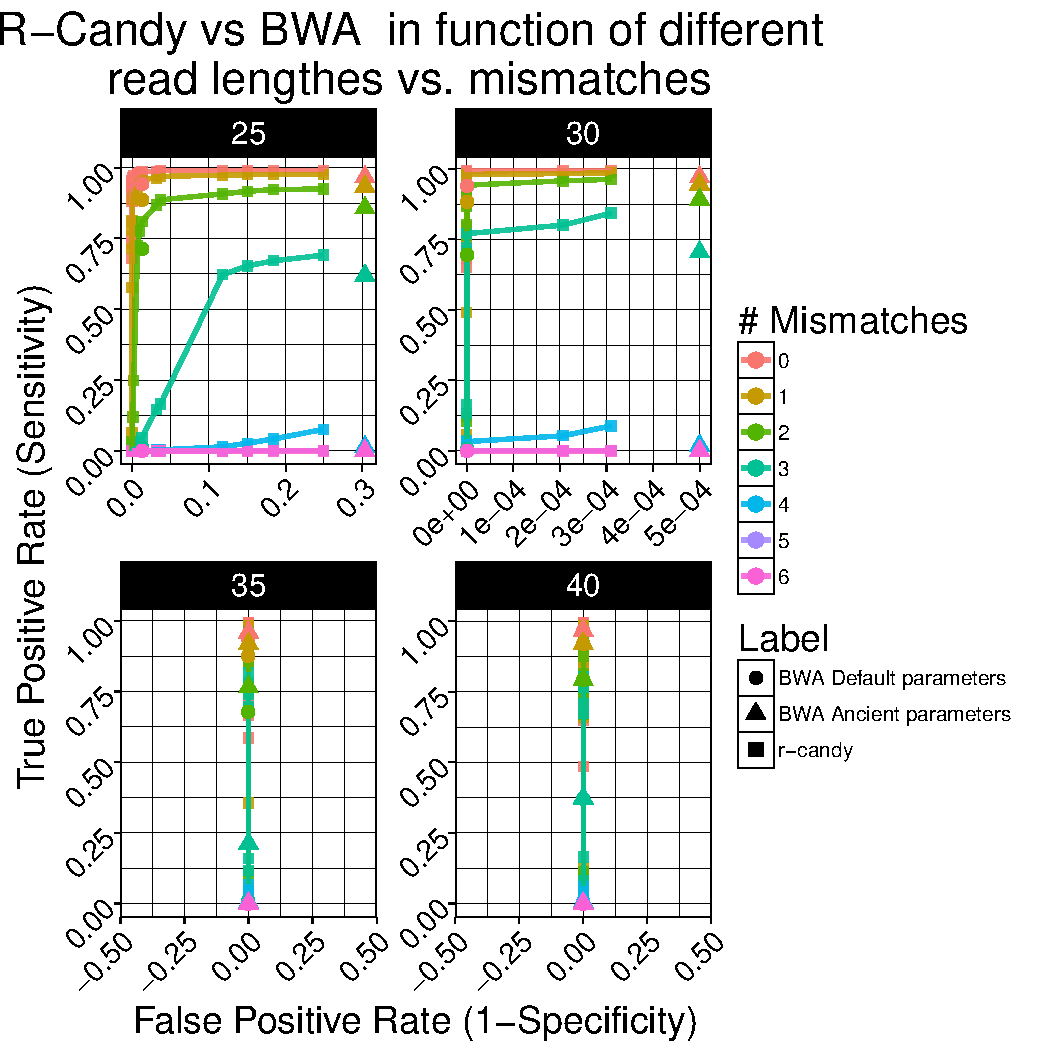
\includegraphics[width=12cm]{pictures/bROC_DS1_emp.pdf}

\caption{
ROC curve for the alignment to the simulated reference genome of simulated ancient 
sequence reads of lengths 25-40bp with damage parameters as explained in Data 
and between 0 and 6 substitutions due to increasing sequence divergence and
empirical sequencing error.
}
\label{DS1_emp}
\end{figure}



The ROC curve shows R-Candy's accuracy under the different alignment score 
cutoffs. As the result shows, R-Candy achieves the highest rate of sensitivity
in all four given lengths.

Reads in length 25 are very challenging for aligners, where
the spurious alignments of contaminant read sequences are very likely.

For deaminated reads of length 25 bps with no divergence substitution 
(the plot with zero mismatches), the sensitivity rate for R-Candy is 99\% 
compare to BWA with ancient-parameters 97\% and BWA with default parameters 94\%. 


For the reads of length 30 bps, the sensitivity values are 98\%, 94\% 
and 88\% for R-Candy, BWA with ancient data parameters and BWA with 
default parameters respectively, which again yields R-Candy's higher
accuracy.

As is expected introducing extra mismatches to the reads decreases  
the sensitivity of the both aligners.

The huge decrease in the false positive rates between reads of length 
25 and 30 shows that even five bases difference can make a huge 
difference in the number of mapped exogenous reads.


No difference in specificity for reads longer than 35 bps is observed
(no microbial reads alignment).


BWA provides more accurate alignments of short 
ancient reads when using the ancient parameters. 
However, with the inclusion of the deamination parameters R-Candy 
outperforms BWA in all cases.


 %%%%%%%%%%%%%%%%%%%%%%%%%%%%%%%%%%%%%%%%%%%%%%%%%%%%%%%%%%%%%%%%%%%%%%%

\subsubsection{Alignment of Simulated Ancient DNA Reads to the Human Reference Genome.}
\label{Alignment of Simulated Ancient DNA Reads to the Human Reference Genome.}
 
 \begin{itemize}
 
    \item \textbf{Data:} Simulated ancient DNA 
     with the following damage parameters $ \sigma = 0.9$, 
    $ \sigma\prime = 0.93 $, $\delta = 0.02 $,  and $\lambda = 0.3 $ and 
    between 0 and 6 substitutions to allow increasing sequence divergence
    including sequencing error generated from empirical quality distribution data
    extracted from a simulated genome.
  
   \item \textbf{Reference genome:} aligned to a the human reference genome (version hg19).

 
    \item \textbf{Aligners:} 
R-Candy with ancient parameters 
(-l left overhang parameter= 0.3, -r right overhang parameter= 0.3 , 
-d deamination rate in double stranded section = 0.02 , 
-s deamination rate in single stranded section = 0.9 )
 and alignments score cut-off of 20. \\
BWA version 0.5.10-evan.10 with default parameters and ancient parameters 
\cite{green2010draft} (the number of mismatches 
(0.01) and the number of gap opens (2)).
 
  \end{itemize}
 

Here we aim to evaluate the performance of R-Candy on ancient DNA reads, 
aligned to the human reference genome with the deamination parameters.


\begin{figure}[H]
\centering
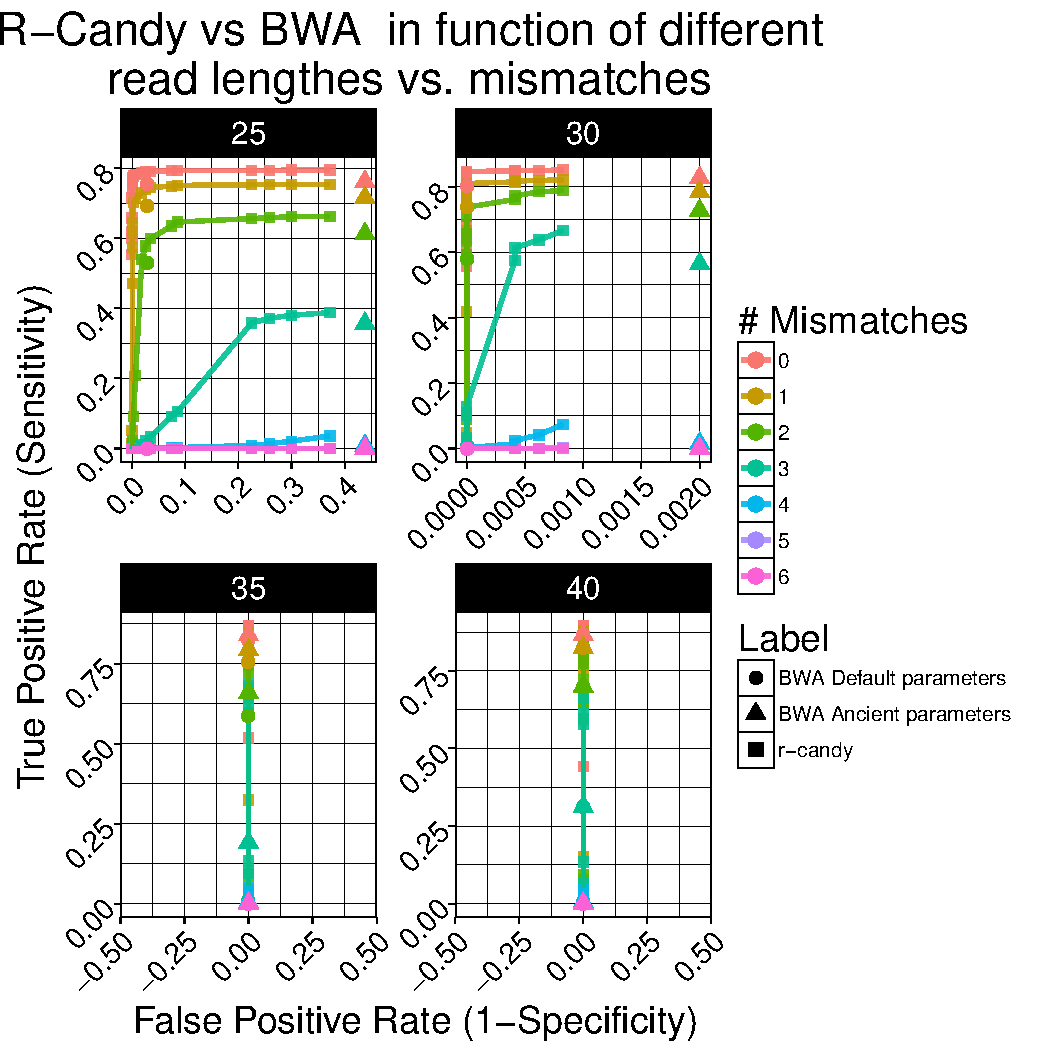
\includegraphics[width=12cm]{pictures/bROC_DS4_emp.pdf}


\caption{
ROC curve for the alignment to the human reference genome of simulated ancient 
sequence reads of lengths 25-40bp with damage parameters as explained in Data 
and between 0 and 6 substitutions due to increasing sequence divergence and
empirical sequencing error.
}

\label{DS4_emp}
\end{figure}

%%%%%%%%%%%%%%%%%%%%%%%%%%%%%%%%%%%%%%%%%%%%%%%%%%%%%%%%%%%%%%%%%%%%%%%%%%%%%%%%%%%%%%%%%%


\subsection{Suitable Alignment Score}
Sensible cut-off from hg19.


%%%%%%%%%%%%%%%%%%%%%%%%%%%%%%%%%%%%%%%%%%%%%%%%%%%%%%%%%%%%%%%%%%%%%%%%%%%%%%%%%%%%%%%%%%%

\subsection{Performance} \label{Performance}

To evaluate R-Candy's speed, we used two test sets, first simulated genomic 
and microbial reads aligned to a simulated genome and second simulated genomic
and microbial reads aligned to a real genome.

The speed evaluation was done on small datasets of 3500 genomic and 1000
microbial reads aligned to a simulated genome of length 1Gbps and the 
human genome of length 3.2 Gbps.

Tables \ref{speed-SG} and \ref{speed-RG} show the speed of 
the two aligners used in this evaluation
R-Candy and BWA both on a single CPU.

Notice that the time required for building the genome index is 
not included in the reported time.\\


\begin{table}[H]
  \begin{tabular}{ |  p{2cm} | p{2cm} | p{3cm} | p{3cm} | }
    \hline
  	\textbf{Type} & \textbf{Read length }&\textbf{Speed BWA \hspace{35pt}(no. of reads/s) } 	 
  	%&\textbf{Speed R-Candy (AS=12, N=1)\hspace{35pt}(no. of reads/s)} 
  	& \textbf{Speed R-Candy AS=20, N=64\hspace{35pt}(no. of reads/s)}\\ \hline
  	  
 	  Genomic    & 25  & 0.0192 &   0.123 \\ \hline
      Genomic    & 30  & 0.0182 &   0.067 \\ \hline
      Genomic    & 35  & 0.0177 &   0.047 \\ \hline
 	  Genomic	 & 40  & 0.0180 &   0.045 \\ \hline
 	  Microbial  & 25  & 0.0629 &   0.540 \\ \hline
      Microbial  & 30  & 0.0619 &   0.319 \\ \hline
 	  Microbial  & 35  & 0.0615 &   0.289 \\ \hline
 	  Microbial  & 40  & 0.0616 &   0.299 \\ \hline
 	  
   \end{tabular}
\caption{The alignment speed for reads aligned to the human reference genome.BWA with default parameters.N = output up to number number of hits per read }
\label{speed-RG}
\end{table}



\begin{table}[h]
  \begin{tabular}{ |  p{2cm} | p{2cm} | p{3cm} | p{3cm} | }
    \hline
  	\textbf{Type} & \textbf{Read length }&\textbf{Speed BWA \hspace{35pt}(no. of reads/s) } 	 
  	%&\textbf{Speed R-Candy (AS=12, N=1)\hspace{35pt}(no. of reads/s)} 
  	& \textbf{Speed R-Candy AS=20, N=64\hspace{35pt}(no. of reads/s)}\\ \hline
  
      Genomic   & 25  & 0.0255  &  0.134 \\ \hline 
      Genomic   & 30  & 0.0248  &  0.066 \\ \hline 
 	  Genomic	& 35  & 0.0237  &  0.066 \\ \hline 
 	  Genomic	& 40  & 0.0244  &  0.059 \\ \hline 
 	  Microbial & 25  & 0.083   &  0.637 \\ \hline 
      Microbial & 30  & 0.0815  &  0.494 \\ \hline 
 	  Microbial & 35  & 0.0810  &  0.477 \\ \hline 
 	  Microbial & 40  & 0.0811  &  0.450 \\ \hline 
 	  
   \end{tabular}
\caption{The alignment speed for reads aligned to the simulated genome.}
\label{speed-SG}
\end{table}



As the results  show  the R-Candy's speed is affected by the read length on both cases.
It decreases from 0.123 number of aligned reads to the human genome per second for reads 
of length 25 bps to 0.045 number of aligned reads per second for reads of length 40 bps. \\
In both test sets, the longer the read is the more running time is required\\

On memory, R-Candy uses 2.5G for single-end mapping.\\

The current version of R-Candy does not support multi-threading to reduce the 
memory usage on multi-core computers.\\\\




%%%%%%%%%%%%%%%%%%%%%%%%%%%%%%%%%%%%%%%%%%%%%%%%%%%%%%%%%%%%%%%%%%%%%%%%%%
%\subsection{Effect Of length on alignment}




%%%%%%%%%%%%%%%%%%%%%%%%%%%%%%%%%%%%%%%%%%%%%%%%%%%%%%%%%%%%%%%%%%%%%

\section{Conclusions} \label{Conclusions}


We have presented R-Candy, a novel method for aligning ancient DNA sequences.
The algorithm for scoring is based on a probabilistic model that takes into account 
the specific characteristics of ancient data, post-mortem deamination damage, as 
well as the other probabilities specific to the data, sequencing error, and species
divergence rate. 
\\
For the both evaluated aligners, varying the cutoff (number of mismatches for BWA 
and alignment score for R-Candy) allows trading a slight increase in sensitivity 
for specificity and runtime.
\\\\
The accuracy of R-Candy on aligning fresh DNA with "default" parameters (no damage model) 
matches BWA, with either "default" or "ancient" parameters, depending  on the cutoff values.
\\\\
R-Candy has a higher sensitivity value on aligning ancient DNA with ancient parameters
compared to BWA with "ancient" parameters and better specificity compared to the 
"default" BWA at the cutoff value of 12.
\\\\
In terms of memory footprint, both aligners are equally good and memory efficient
to load genome. But R-Candy has a very low throughput ratio (speed) compared to 
BWA which makes it unusable in case of big-data and genome of mammalian size. 
\\\\
The main conclusion is R-Candy drags down the shortcut on aDNA alignment to 25 bps 
which it was in lower-bound 35 bps and makes it possible to align more rare and 
low-quality endogenous reads but needs some modifications in terms of speed to 
make it useable on datasets of the size typically generated during ancient human
genome sequencing projects. 



 
%%%%%%%%%%%%%%%%%%%%%%%%%%%%%%%%%%%%%%%%%%%%%%%%%%%%%%%%%%%%%%%%%%%%%%

\section{Future Work} \label{Future Work}
We have shown that for the alignment of ancient DNA reads between 25-40 
bps R-Candy provides superior accuracy to BWA.  
However, a number of points need to be addressed before R-Candy can be used 
on big datasets of ancient genome projects. 

%To increase R-Candy's speed  ...

The backtracking algorithm used by R-Candy is its bottleneck if mismatches 
appear early in the alignment. 
Therefore, alignment of aDNA reads should start from the middle of the read 
out, which requires a different index structure (Bi-directional Wavelet tree).

Applying a seed strategy where the middle part of a read would serve as seed
due to low deamination damage rate in the middle of  ancient DNA read sequences.

Distribute or parallel the program and support multithreading feature.

A method that combines dynamic programming with a Full-Text index might extend
the usefulness of R-Candy to longer reads.

%%%%%%%%%%%%%%%%%%%%%%%%%%%%%%%%%%%%%%%%%%%%%%%%%%%%%%%%%%%%%%%%%%%%%%

\section{Availability} \label{Availability}

R-Candy's documentation and source code are freely available at\\
 (https://github.com/udo-stenzel/r-candy.git).
\\\\
Genome/read simulation program written in C++ is freely available at
(https://github.com/Homa1127/simulateGenome.git).
\\\\
The hash program for analysing R-Candy's output written in C++, available at
https://github.com/Homa1127/rcandyHash.git



%%%%%%%%%%%%%%%%%%%%%%%%%%%%%%%%%%%%%%%%%%%%%%%%%%%%%%%%%%%%%%%%%%%%%%%%

\section{Abbreviations} \label{Abbreviations}

\textbf{DNA}: deoxyribonucleic acid;
\textbf{bp}: base pair;
\textbf{NGS}: next generation sequencing technologies;
\textbf{BWT}: Burrows-Wheeler transform;
\textbf{FM}: full-text minute-space;
\textbf{A}: Adenine;
\textbf{C}: Cytosine;
\textbf{T}: Thymine;
\textbf{G}: Guanine;
\textbf{PacBio}: Pacific Bioscience;
\textbf{SA}: suffix array;
\textbf{LF}: last to first;
\textbf{DFS}: depth first search;
\textbf{DP}: dynamic programming;
\textbf{BAM}: Binary Alignment/Map;
\textbf{CDF}: cumulative distribution function.
\textbf{PCR}: Polymerase Chain Reaction.



%%%%%%%%%%%%%%%%%%%%%%%%%%%%%%%%%%%%%%%%%%%%%%%%%%%%%%%%%%%%%%%%%%%%%

\newpage
\appendix
\section*{Appendix}
\renewcommand{\thesubsection}{\Alph{subsection}}

\subsection{Simulation sequencing error by ART software} 
\label{Simulation sequencing error by ART software}

In this section, I follow all the evaluation scenarios which I explained in
Section \ref{Evaluation Scenarios}  with different sequencing error simulation.
ART, a next-generation sequencing read simulator is used to simulate sequencing
error of Illumina platform. 
ART generates sequencing reads based on different sequencing technology 
platforms (454, Illumina, SOLiD) criteria[35] and simulates the
substitution error probability, based on the base-quality 
score distribution reported by large training datasets[35].\\

In order to use ART in readSim user needs to specify the sequencing
platform and the reads length for generating base quality scores.\\

The result of aligning different datasets showed that ART simulates a
low base quality score (compared to the empirical data) that leads to 
a high rate of sequencing error which degrades the performance of BWA.\\

So we didn't use it for our evaluations. \\

\begin{figure}[H]
\centering
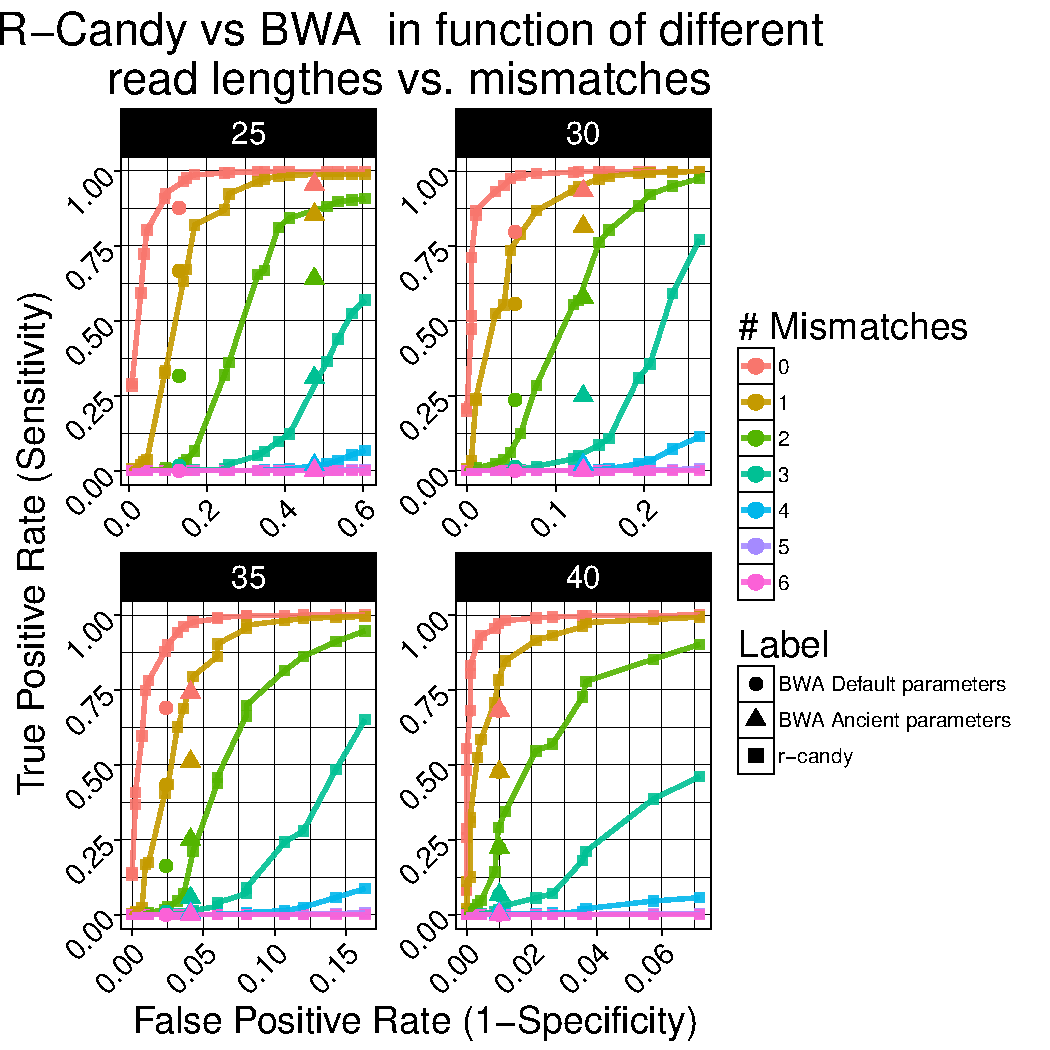
\includegraphics[width=12cm]{pictures/bROC_DS3_ART.pdf}
\caption{
ROC curve for the alignment to the simulated reference genome of simulated fresh 
sequence reads of lengths 25-40bp with between 0 and 6 substitutions due 
to increasing sequence divergence and sequencing error by ART.}
\label{DS3_ART}
\end{figure}



\begin{figure}[H]
\centering
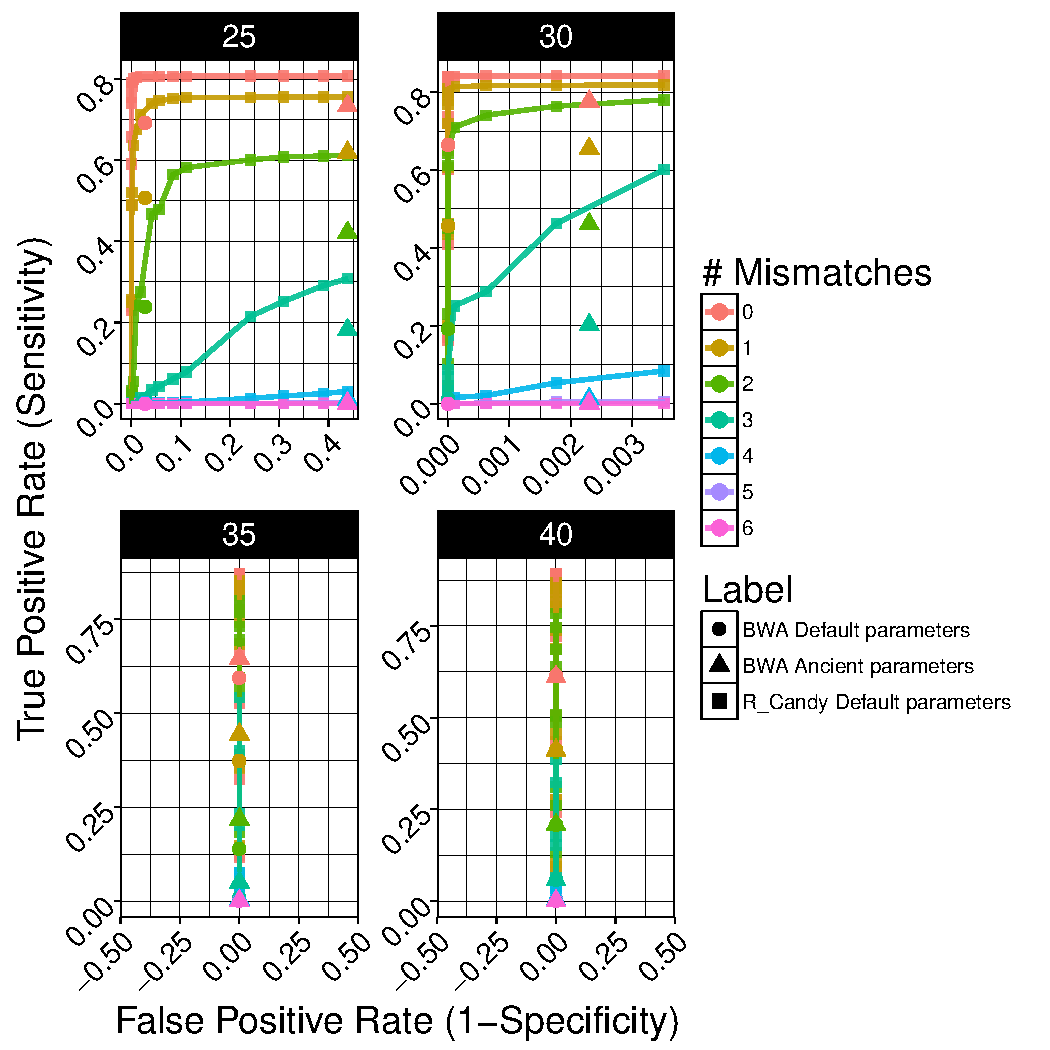
\includegraphics[width=12cm]{pictures/bROC_DS6_ART.pdf}
\caption{
ROC curve for the alignment to the human reference genome of simulated fresh 
sequence reads of lengths 25-40bp with between 0 and 6 substitutions due 
to increasing sequence divergence and sequencing error by ART.
}
\label{DS6_ART}
\end{figure}



\begin{figure}[H]
\centering
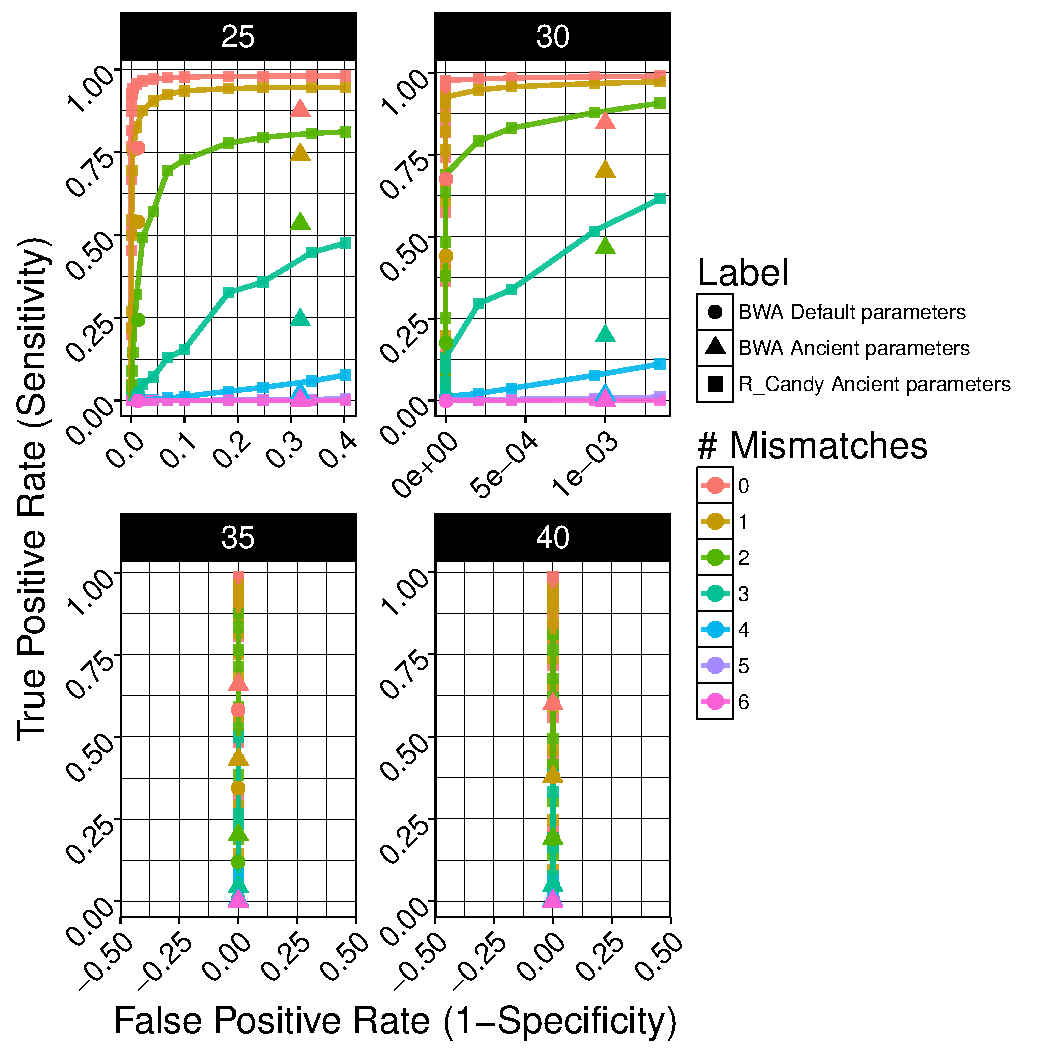
\includegraphics[width=12cm]{pictures/bROC_DS1_ART.pdf}
\caption{
ROC curve for the alignment to the simulated reference genome of simulated ancient 
sequence reads of lengths 25-40bp with damage parameters as explained in Data 
and between 0 and 6 substitutions due to increasing sequence divergence and
empirical sequencing error.
}
\label{DS1_ART}
\end{figure}



\begin{figure}[H]
\centering
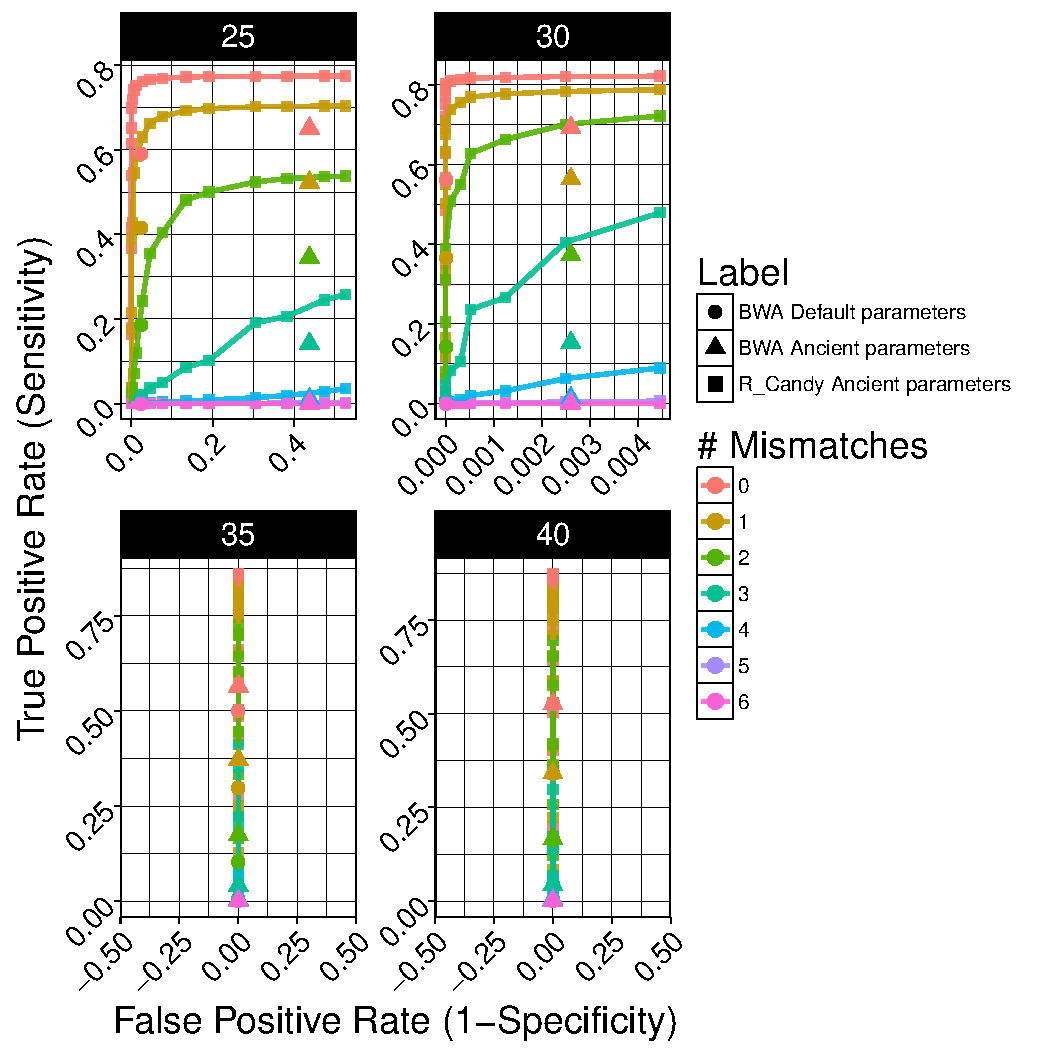
\includegraphics[width=12cm]{pictures/bROC_DS4_ART.pdf}
\caption{
ROC curve for the alignment to the human reference genome of simulated ancient 
sequence reads of lengths 25-40bp with damage parameters as explained in Data 
and between 0 and 6 substitutions due to increasing sequence divergence and
empirical sequencing error.
}
\label{DS4_ART}
\end{figure}



%%%%%%%%%%%%%%%%%%%%%%%%%%%%%%%%%%%%%%%%%%%%%%%%%%%%%%%%%%%%%%%%%%%%
\bibliographystyle{unsrt}
\bibliography{Ref}


\end{document} 
   
      
      
              
